\documentclass [aspectratio=169]{beamer}
\beamertemplatenavigationsymbolsempty
\usetheme{Boadilla}
\usepackage{textpos} % package for the positioning
\usepackage[]{graphicx}
\usepackage{graphicx}
\usepackage{float}
\usepackage{hyperref}
\usepackage{caption}
\usepackage{subcaption}
\usepackage{algorithm,algpseudocode}
\usepackage[export]{adjustbox}
\usepackage{tikz}
\usepackage[square,numbers]{natbib}
\usepackage[byname]{smartref}
\usetikzlibrary{positioning}
\usetikzlibrary{arrows, shapes, decorations, automata, backgrounds, fit, petri, calc}

\newcommand*{\logofont}{\fontfamily{phv}\selectfont}

\definecolor{uwopurple}{RGB}{79,38,131} % official purple color for uwo

\title[]{\vspace{60pt} \\
Traum und Wirklichkeit} % Change the lecture topic right here!
\subtitle{From Berkeley to Canfranc}
\author[]{J.J. Gómez Cadenas}
\institute[]{Donostia International Physics Center}
\date{\today}

% Math notations
\newtheorem{thm}{Theorem}[section]
\newtheorem{lem}[thm]{Lemma}

\newtheorem{defn}[thm]{Definition}
\newtheorem{eg}[thm]{Example}
\newtheorem{ex}[thm]{Exercise}
\newtheorem{conj}[thm]{Conjecture}
\newtheorem{cor}[thm]{Corollary}
\newtheorem{claim}[thm]{Claim}
\newtheorem{rmk}[thm]{Remark}

\newcommand{\ie}{\emph{i.e.} }
\newcommand{\cf}{\emph{cf.} }
\newcommand{\into}{\hookrightarrow}
\newcommand{\dirac}{\slashed{\partial}}
\newcommand{\bbonu}{\ensuremath{\beta\beta0\nu}}
\newcommand{\bbtnu}{\ensuremath{\beta\beta2\nu}}
\newcommand{\mbb}{\ensuremath{m_{\beta\beta}}}
\newcommand{\qbb}{\ensuremath{Q_{\beta\beta}}}
\newcommand{\mbbsq}{\ensuremath{m_{\beta\beta}^2}}
\newcommand{\tonu}{\ensuremath{(T_{1/2}^{0\nu})^{-1}}}
\newcommand{\gonu}{\ensuremath{G^{0\nu}}}
\newcommand{\monu}{\ensuremath{| M^{0\nu}|^2}}
\newcommand{\XE}{\ensuremath{{}^{136}{\rm Xe}}}
\newcommand{\GE}{\ensuremath{{}^{76}{\rm Ge}}}
\newcommand{\TE}{\ensuremath{{}^{130}{\rm Te}}}
\newcommand{\TL}{\ensuremath{{}^{208}{\rm Tl}}}
\newcommand{\BI}{\ensuremath{{}^{214}{\rm Bi}}}
\newcommand{\MO}{\ensuremath{{}^{100}{\rm Mo}}}
\newcommand{\KR}{\ensuremath{{}^{83}{\rm Kr}}}
\newcommand{\nne}{\ensuremath{\bar{N}_e}}
\newcommand{\nng}{\ensuremath{\bar{N}_\gamma}}
\newcommand{\so}{\ensuremath{\rm S_1}}
\newcommand{\st}{\ensuremath{\rm S_2}}
\newcommand{\tz}{\ensuremath{\rm t_0}}
\newcommand{\R}{\mathbb{R}}
\newcommand{\C}{\mathbb{C}}
\newcommand{\Z}{\mathbb{Z}}
\newcommand{\N}{\mathbb{N}}
\newcommand{\Q}{\mathbb{Q}}
\newcommand{\LieT}{\mathfrak{t}}
\newcommand{\T}{\mathbb{T}}
\newcommand{\A}{\mathds{A}}
\newcommand{\E}{\mathbb{E}}
\newcommand{\Prob}{\mathbb{P}}
\newcommand{\Var}{\text{Var}}
\newcommand\equalhat{%
\let\savearraystretch\arraystretch
\renewcommand\arraystretch{0.3}
\begin{array}{c}
\stretchto{
    \scalerel*[\widthof{=}]{\wedge}
    {\rule{1ex}{3ex}}%
}{0.5ex}\\ 
=%
\end{array}
\let\arraystretch\savearraystretch
}

% set color
\setbeamercolor{title in head/foot}{bg=white}
\setbeamercolor{author in head/foot}{bg=white}
\setbeamercolor{date in head/foot}{fg=uwopurple}
\setbeamercolor{date in head/foot}{bg=white}
\setbeamercolor{title}{fg=uwopurple}
\setbeamerfont{title}{series=\bfseries}
\setbeamercolor{frametitle}{fg=uwopurple}
\setbeamerfont{frametitle}{series=\bfseries}
\setbeamercolor{block title}{bg=uwopurple!30,fg=black}
\setbeamercolor{item}{fg=uwopurple}
\setbeamercolor{caption name}{fg=uwopurple!70!}


% set logo at non-title pages
%\logo{
\includegraphics[height=0.9cm]{dipc.png}\vspace*{-.45\paperheight}\hspace*{.50\paperwidth}}

\begin{document}

{
\setbeamertemplate{logo}{}
\begin{frame}
    \titlepage
    \begin{textblock*}{4cm}(0.5cm,-7.3cm)
        
\includegraphics[width=4cm]{dipc.png}
    \end{textblock*}
    \begin{textblock*}{8cm}(5.0cm,-7.0cm)
        \huge \color{uwopurple}{$\Bigr\rvert$ \hspace{0.15cm} \textbf{Lecture 4}} % Change the lecture # right here! 
    \end{textblock*}
\end{frame}
}

%%%%
\begin{frame}{A meeting in Berkeley}

\begin{columns}
\column{0.60\textwidth}
\includegraphics[scale=0.06]{berkely.png}


 \column{0.40\textwidth}
$\bullet~$ {\bf Dream and reality}. In 2009, Dave Nygren, James White \& JJ, met at Berkeley, and NEXT was born, as least as a {\em traum}. The lessons from St. Gotthard TPC were that the topological signature was available, but one had to keep \so\ for fiducialisation and improve on energy resolution.    

\end{columns}
\end{frame}


\begin{frame}{The conceptual design}

\begin{columns}
\column{0.60\textwidth}
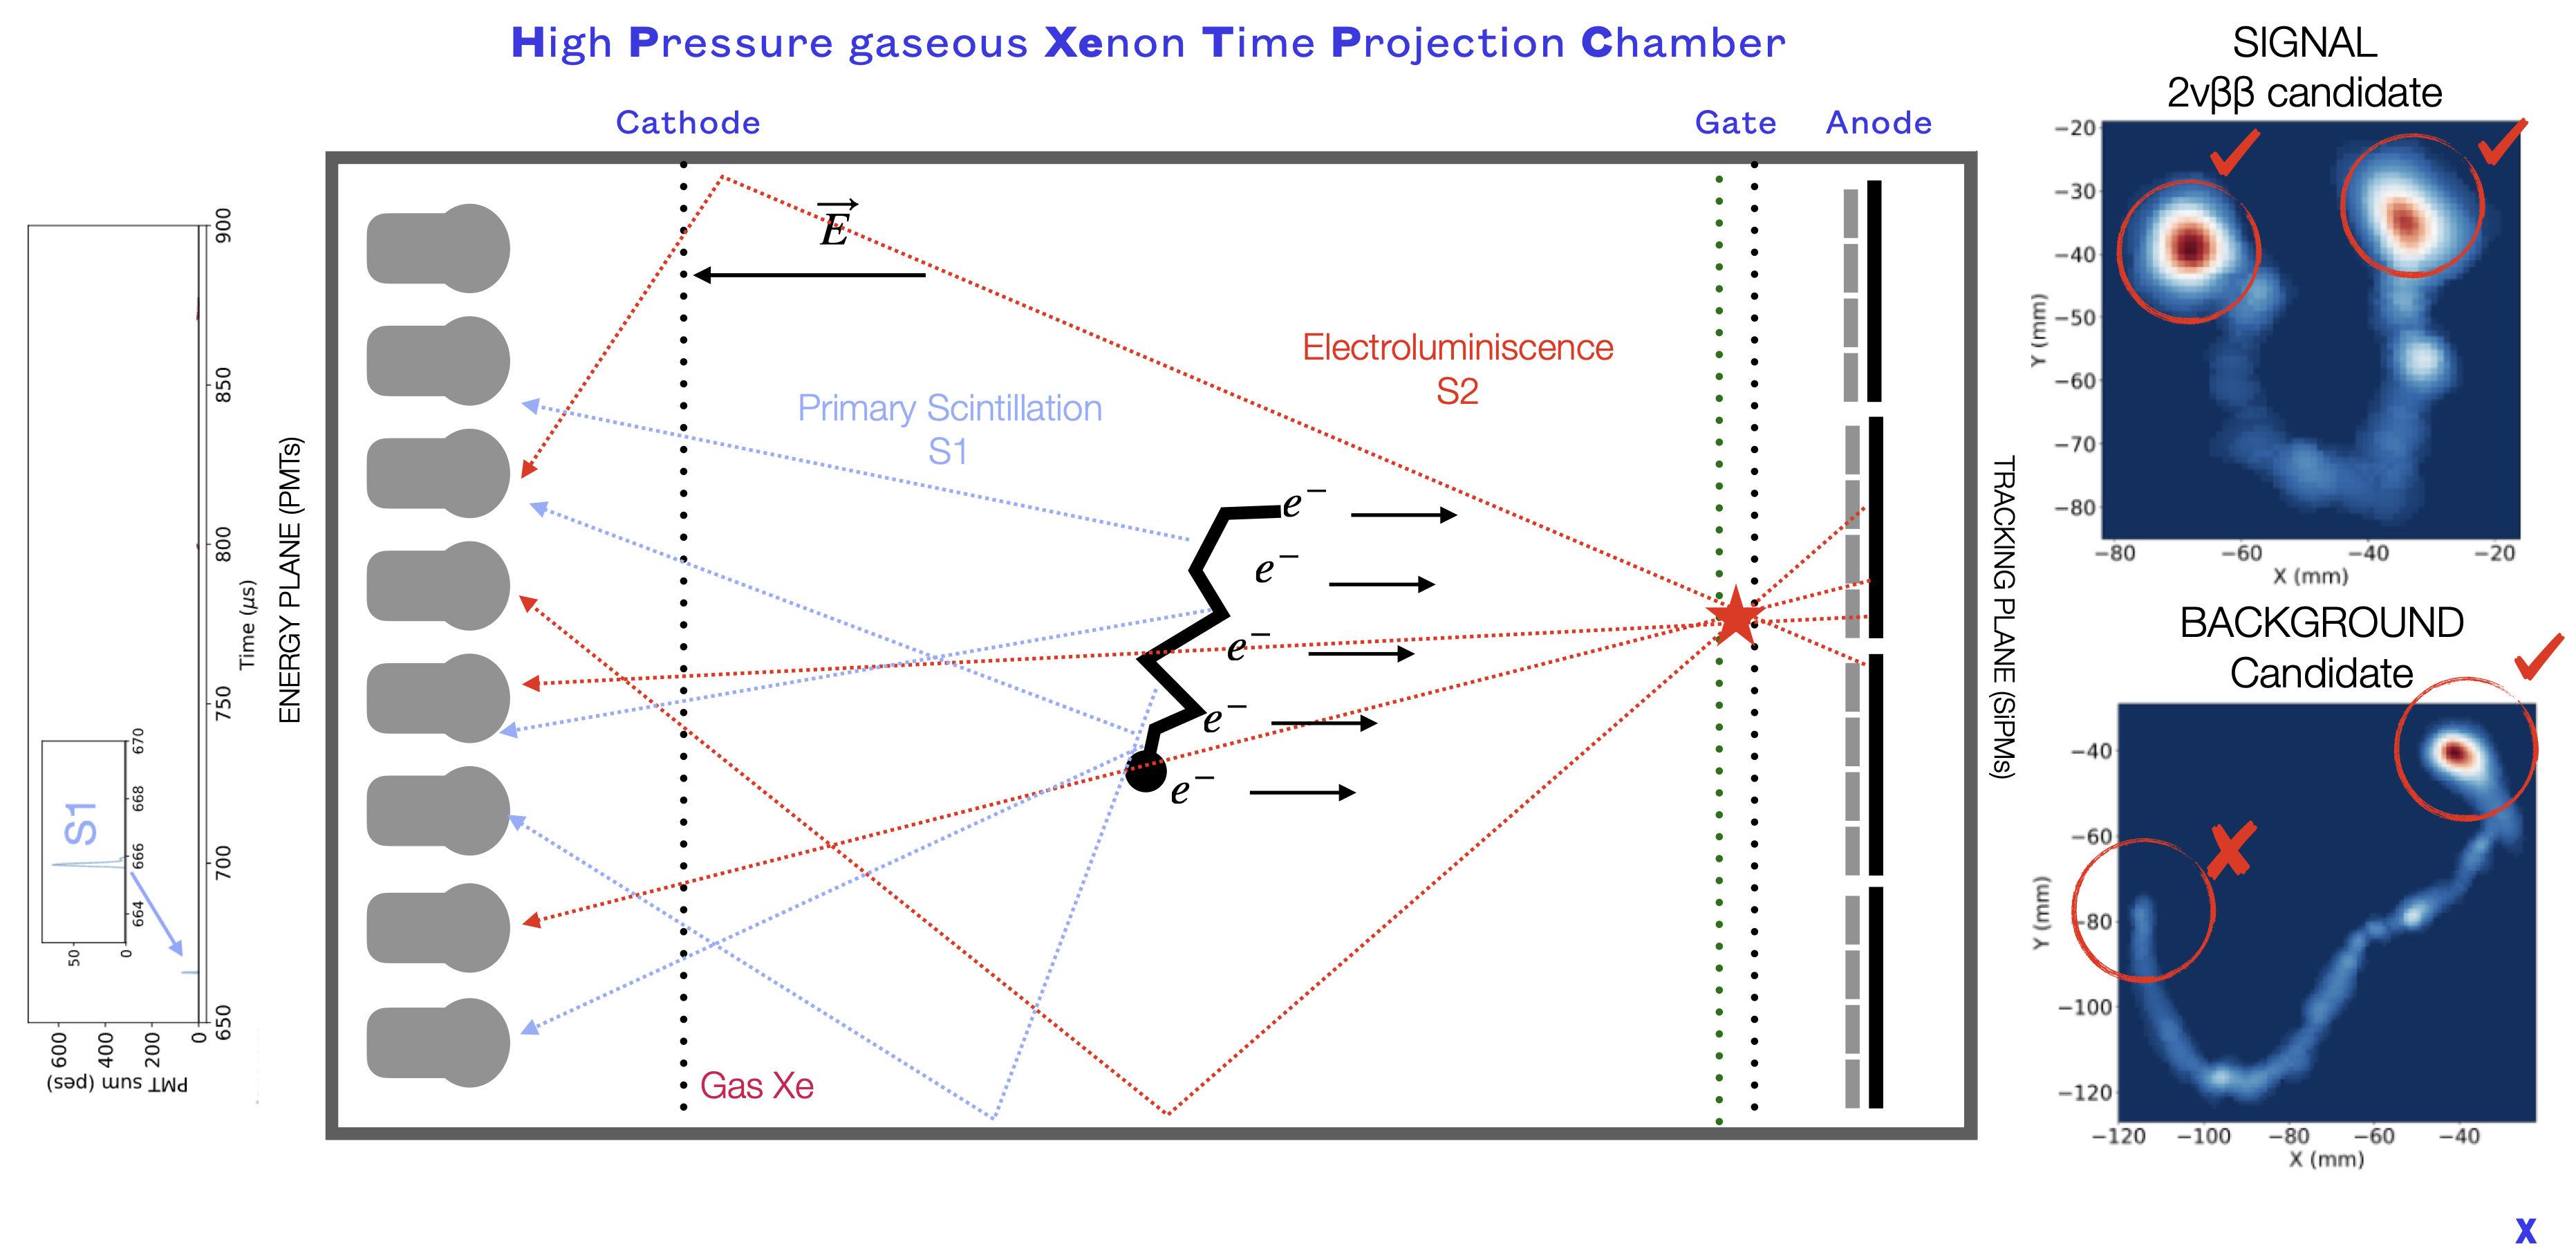
\includegraphics[scale=0.14]{nexttraum.png}


 \column{0.40\textwidth}
$\bullet~$ NEXT  was originally conceived as a EL TPC (energy resolution, \so\ available), with an energy plane (PMTs to integrate as much as the emitted signal as possible) and a tracking plane (made os SiPMs in order to pixelise the track) was born.  

$\bullet~$ The working pressure could be anything between 5-20 bar. High pressure allows more mass per unit volume, but implies higher electric fields and more diffusion, thus, potentially weakening the topological signature. 

\end{columns}
\end{frame}

%%%
\begin{frame}{Early Prototypes}

\begin{columns}
\column{0.60\textwidth}
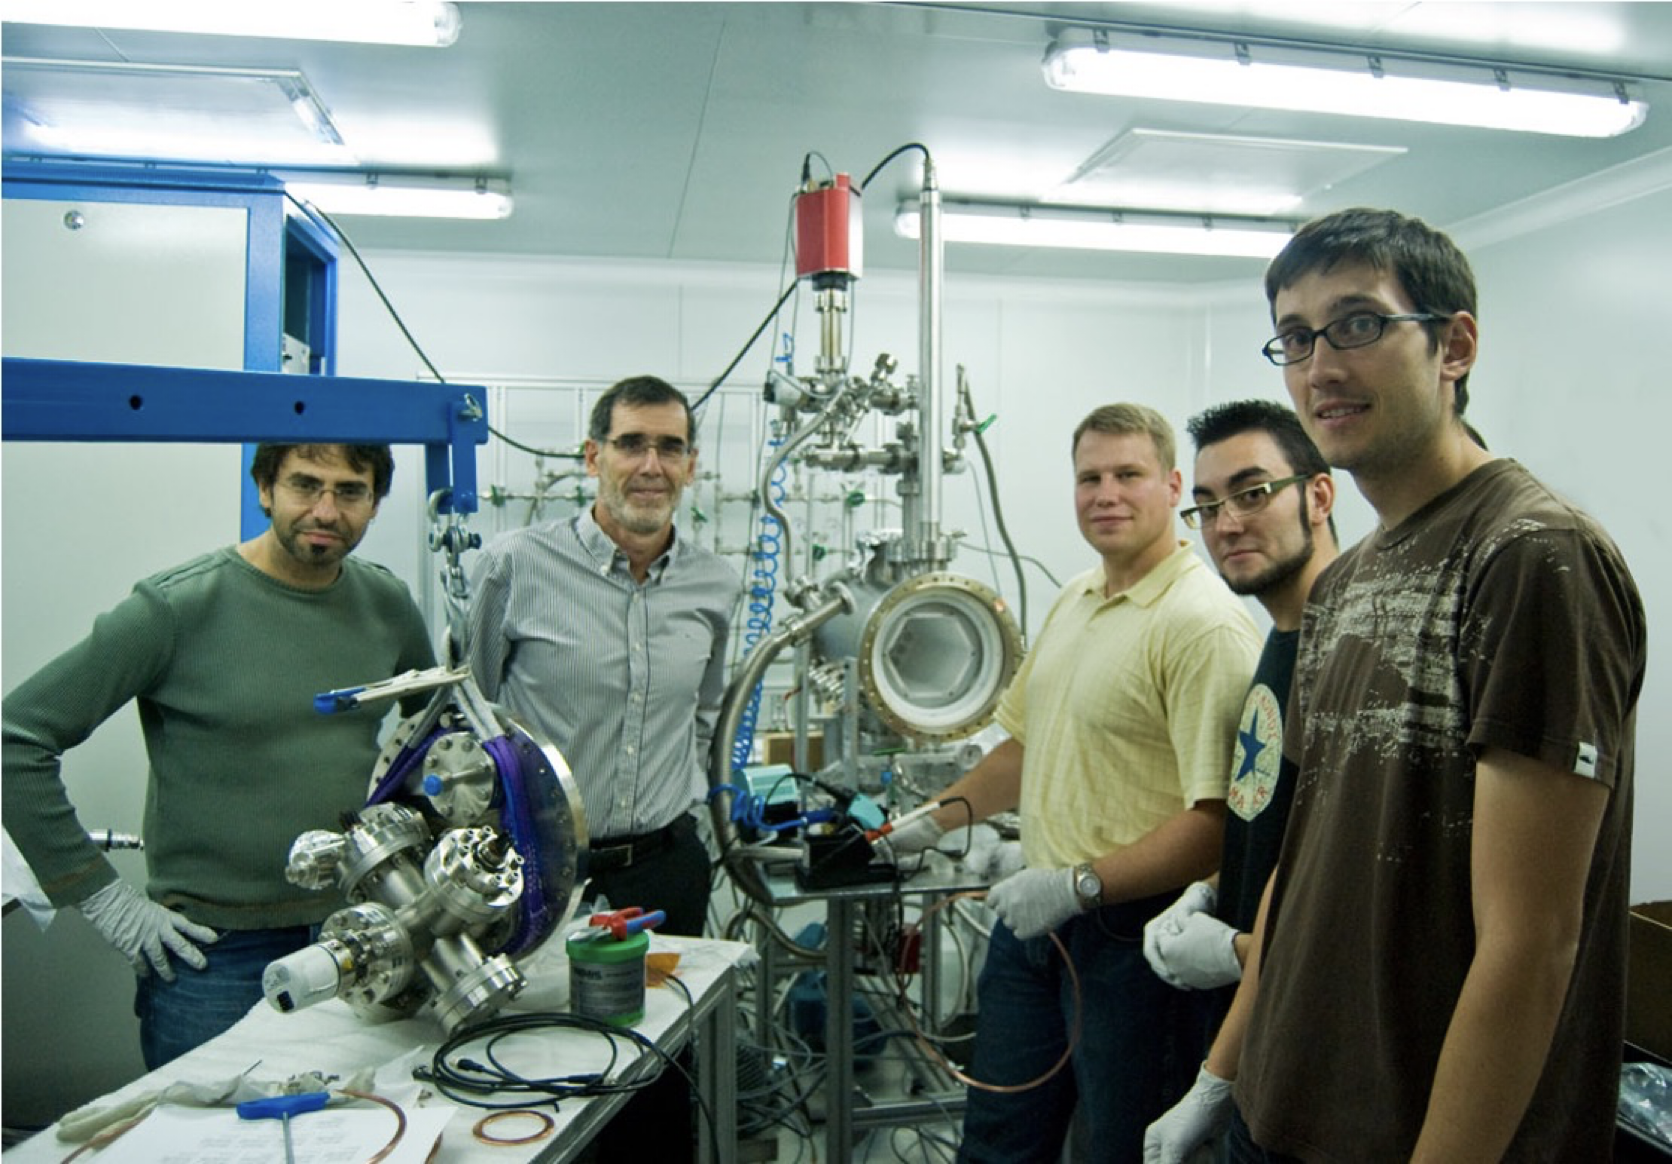
\includegraphics[scale=0.28]{next-demo.png}


 \column{0.40\textwidth}
$\bullet~$ Between 2009 and 2015 we operated two prototypes. DBDM at LBNL (refer to previous lectures) and NEXT-DEMO at IFIC, in Spain. {\em Traum} became {\em Wirklichkeit}.

\end{columns}
\end{frame}

\begin{frame}{NEXT-White}

\begin{columns}
\column{0.60\textwidth}
\includegraphics[scale=0.11]{white.png}

 \column{0.40\textwidth}
$\bullet~$ NEXT-White (name in loving memory of James), was the first radiopure NEXT-detector. It operated at the LSC (Canfranc) from 2016 to 2022.

\end{columns}
\end{frame}

\begin{frame}{Anatomy of NEXT-White}

\begin{columns}
\column{0.60\textwidth}
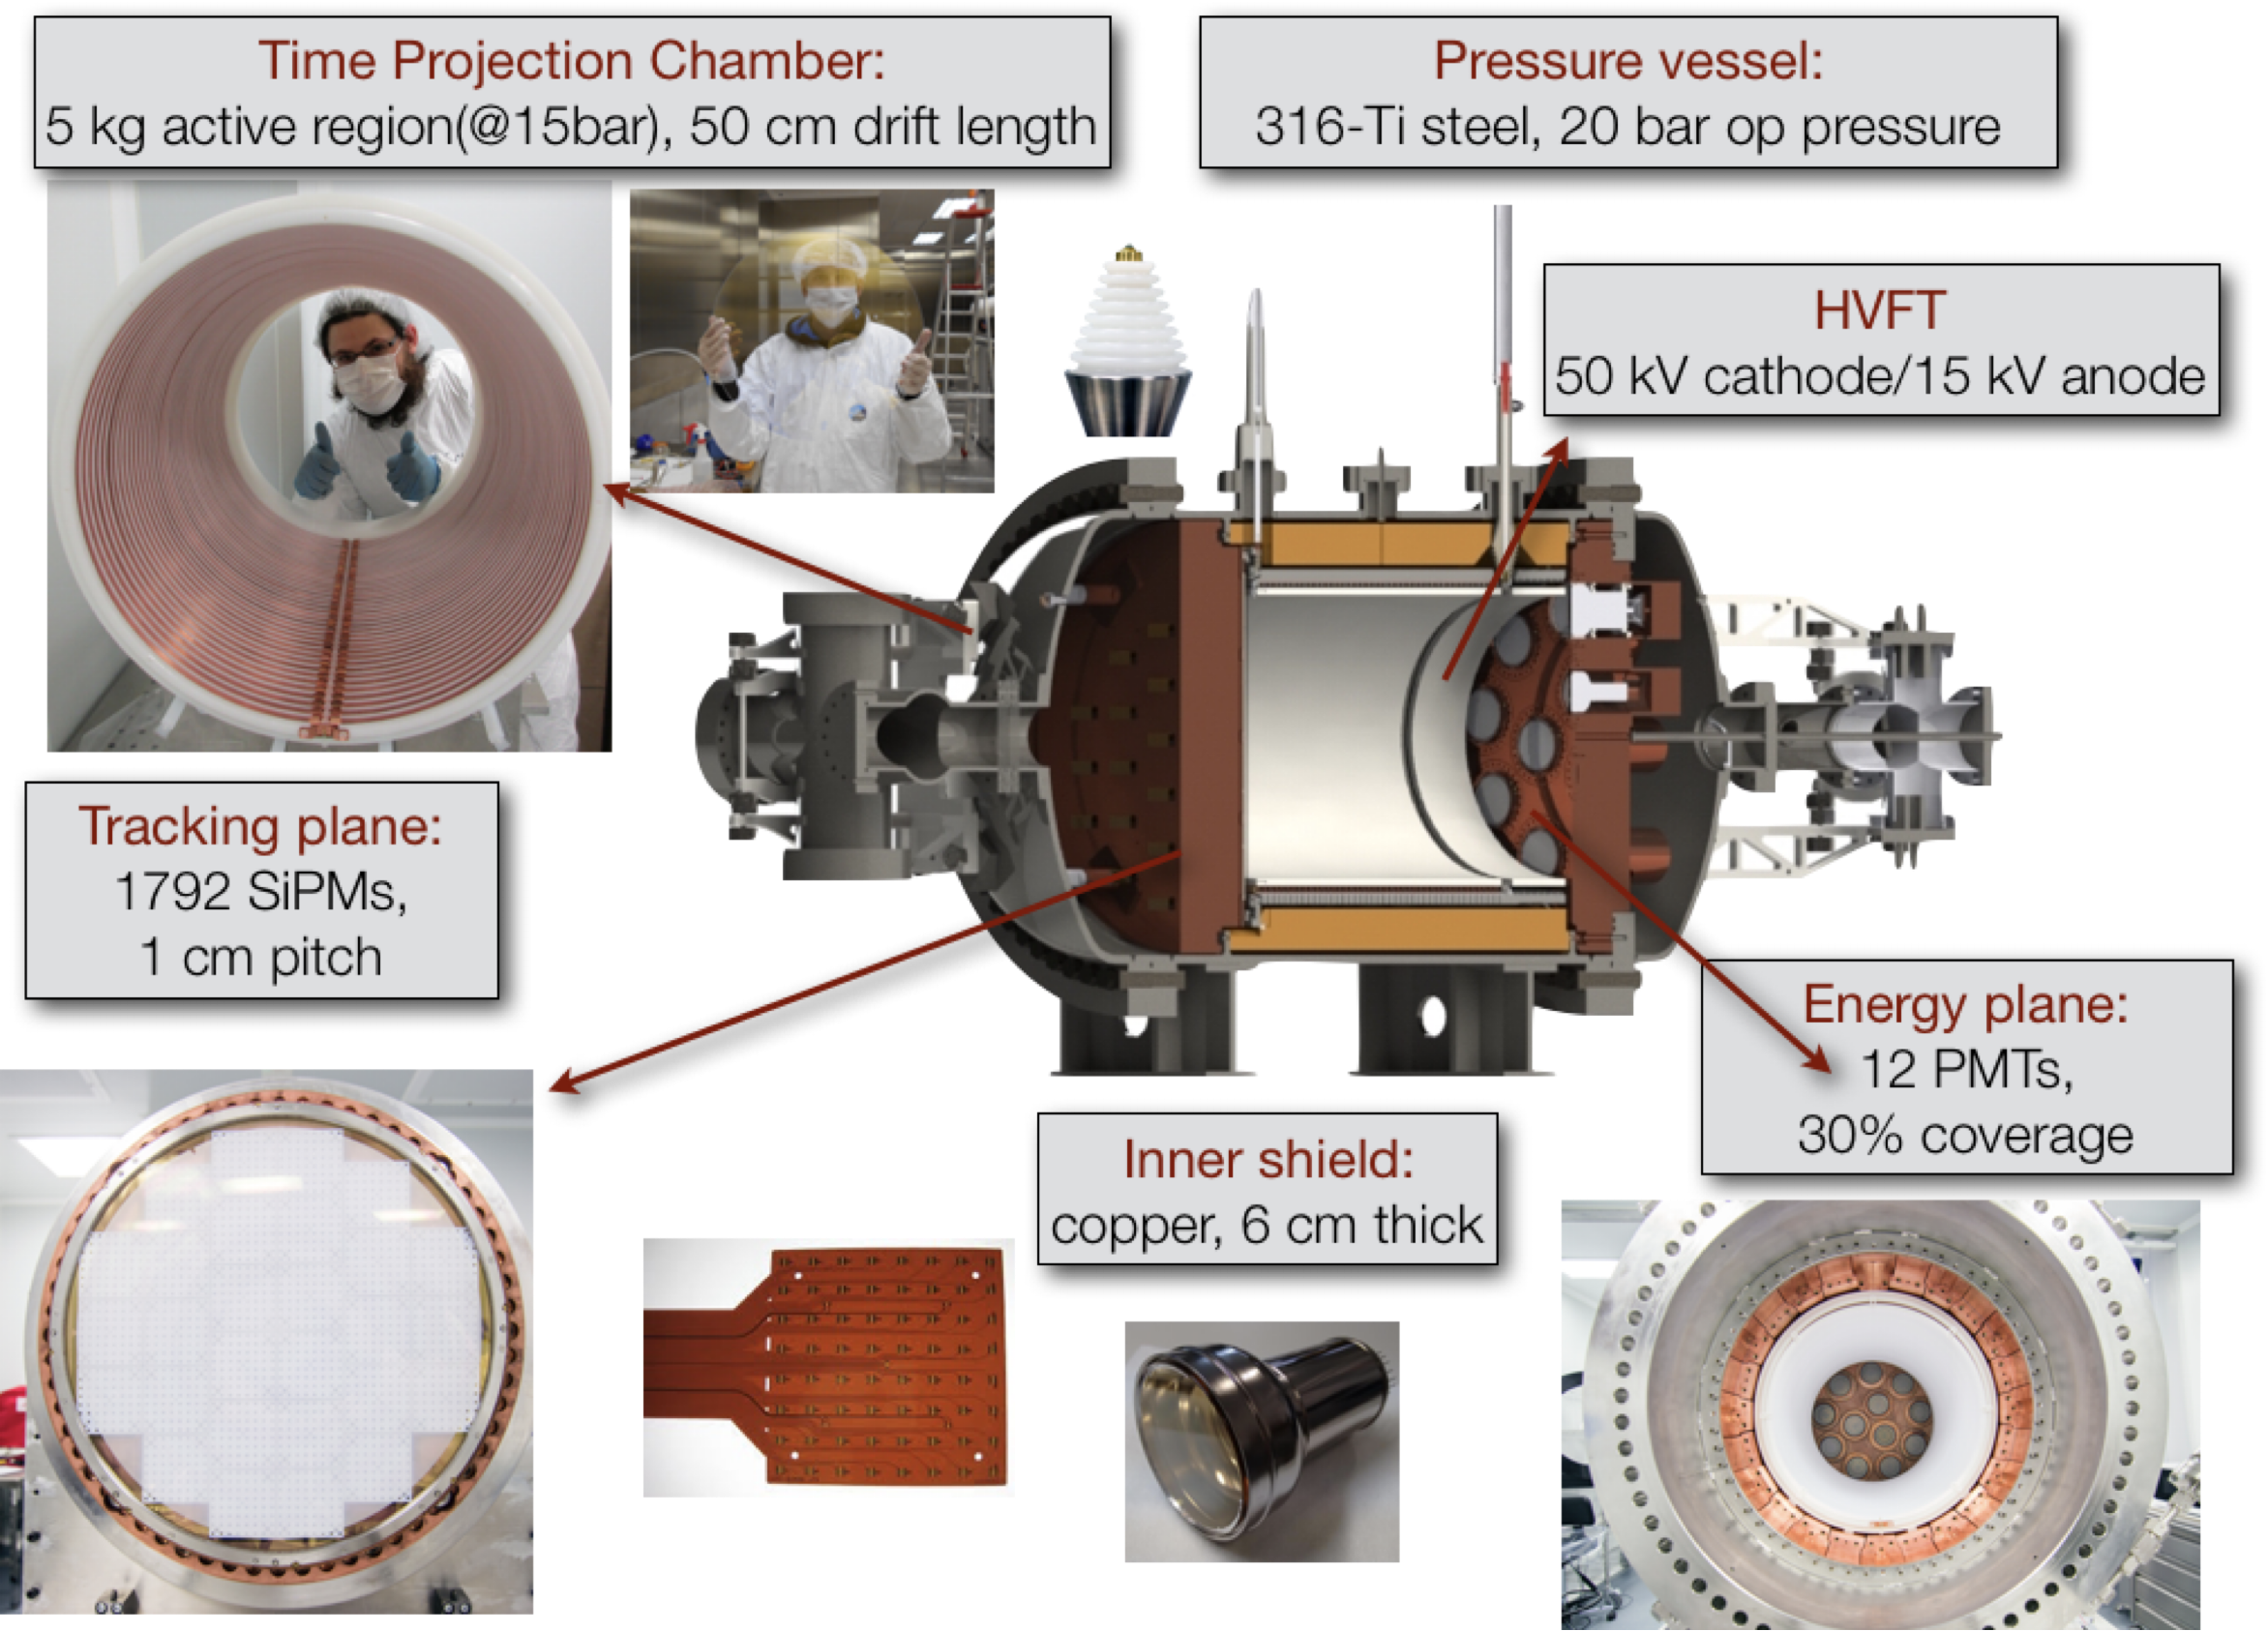
\includegraphics[scale=0.21]{whitecollage.png}

 \column{0.40\textwidth}
$\bullet~$ NEXT-White was a full implementation of the (original) NEXT concept. 

\end{columns}
\end{frame}

\begin{frame}{Energy Plane}

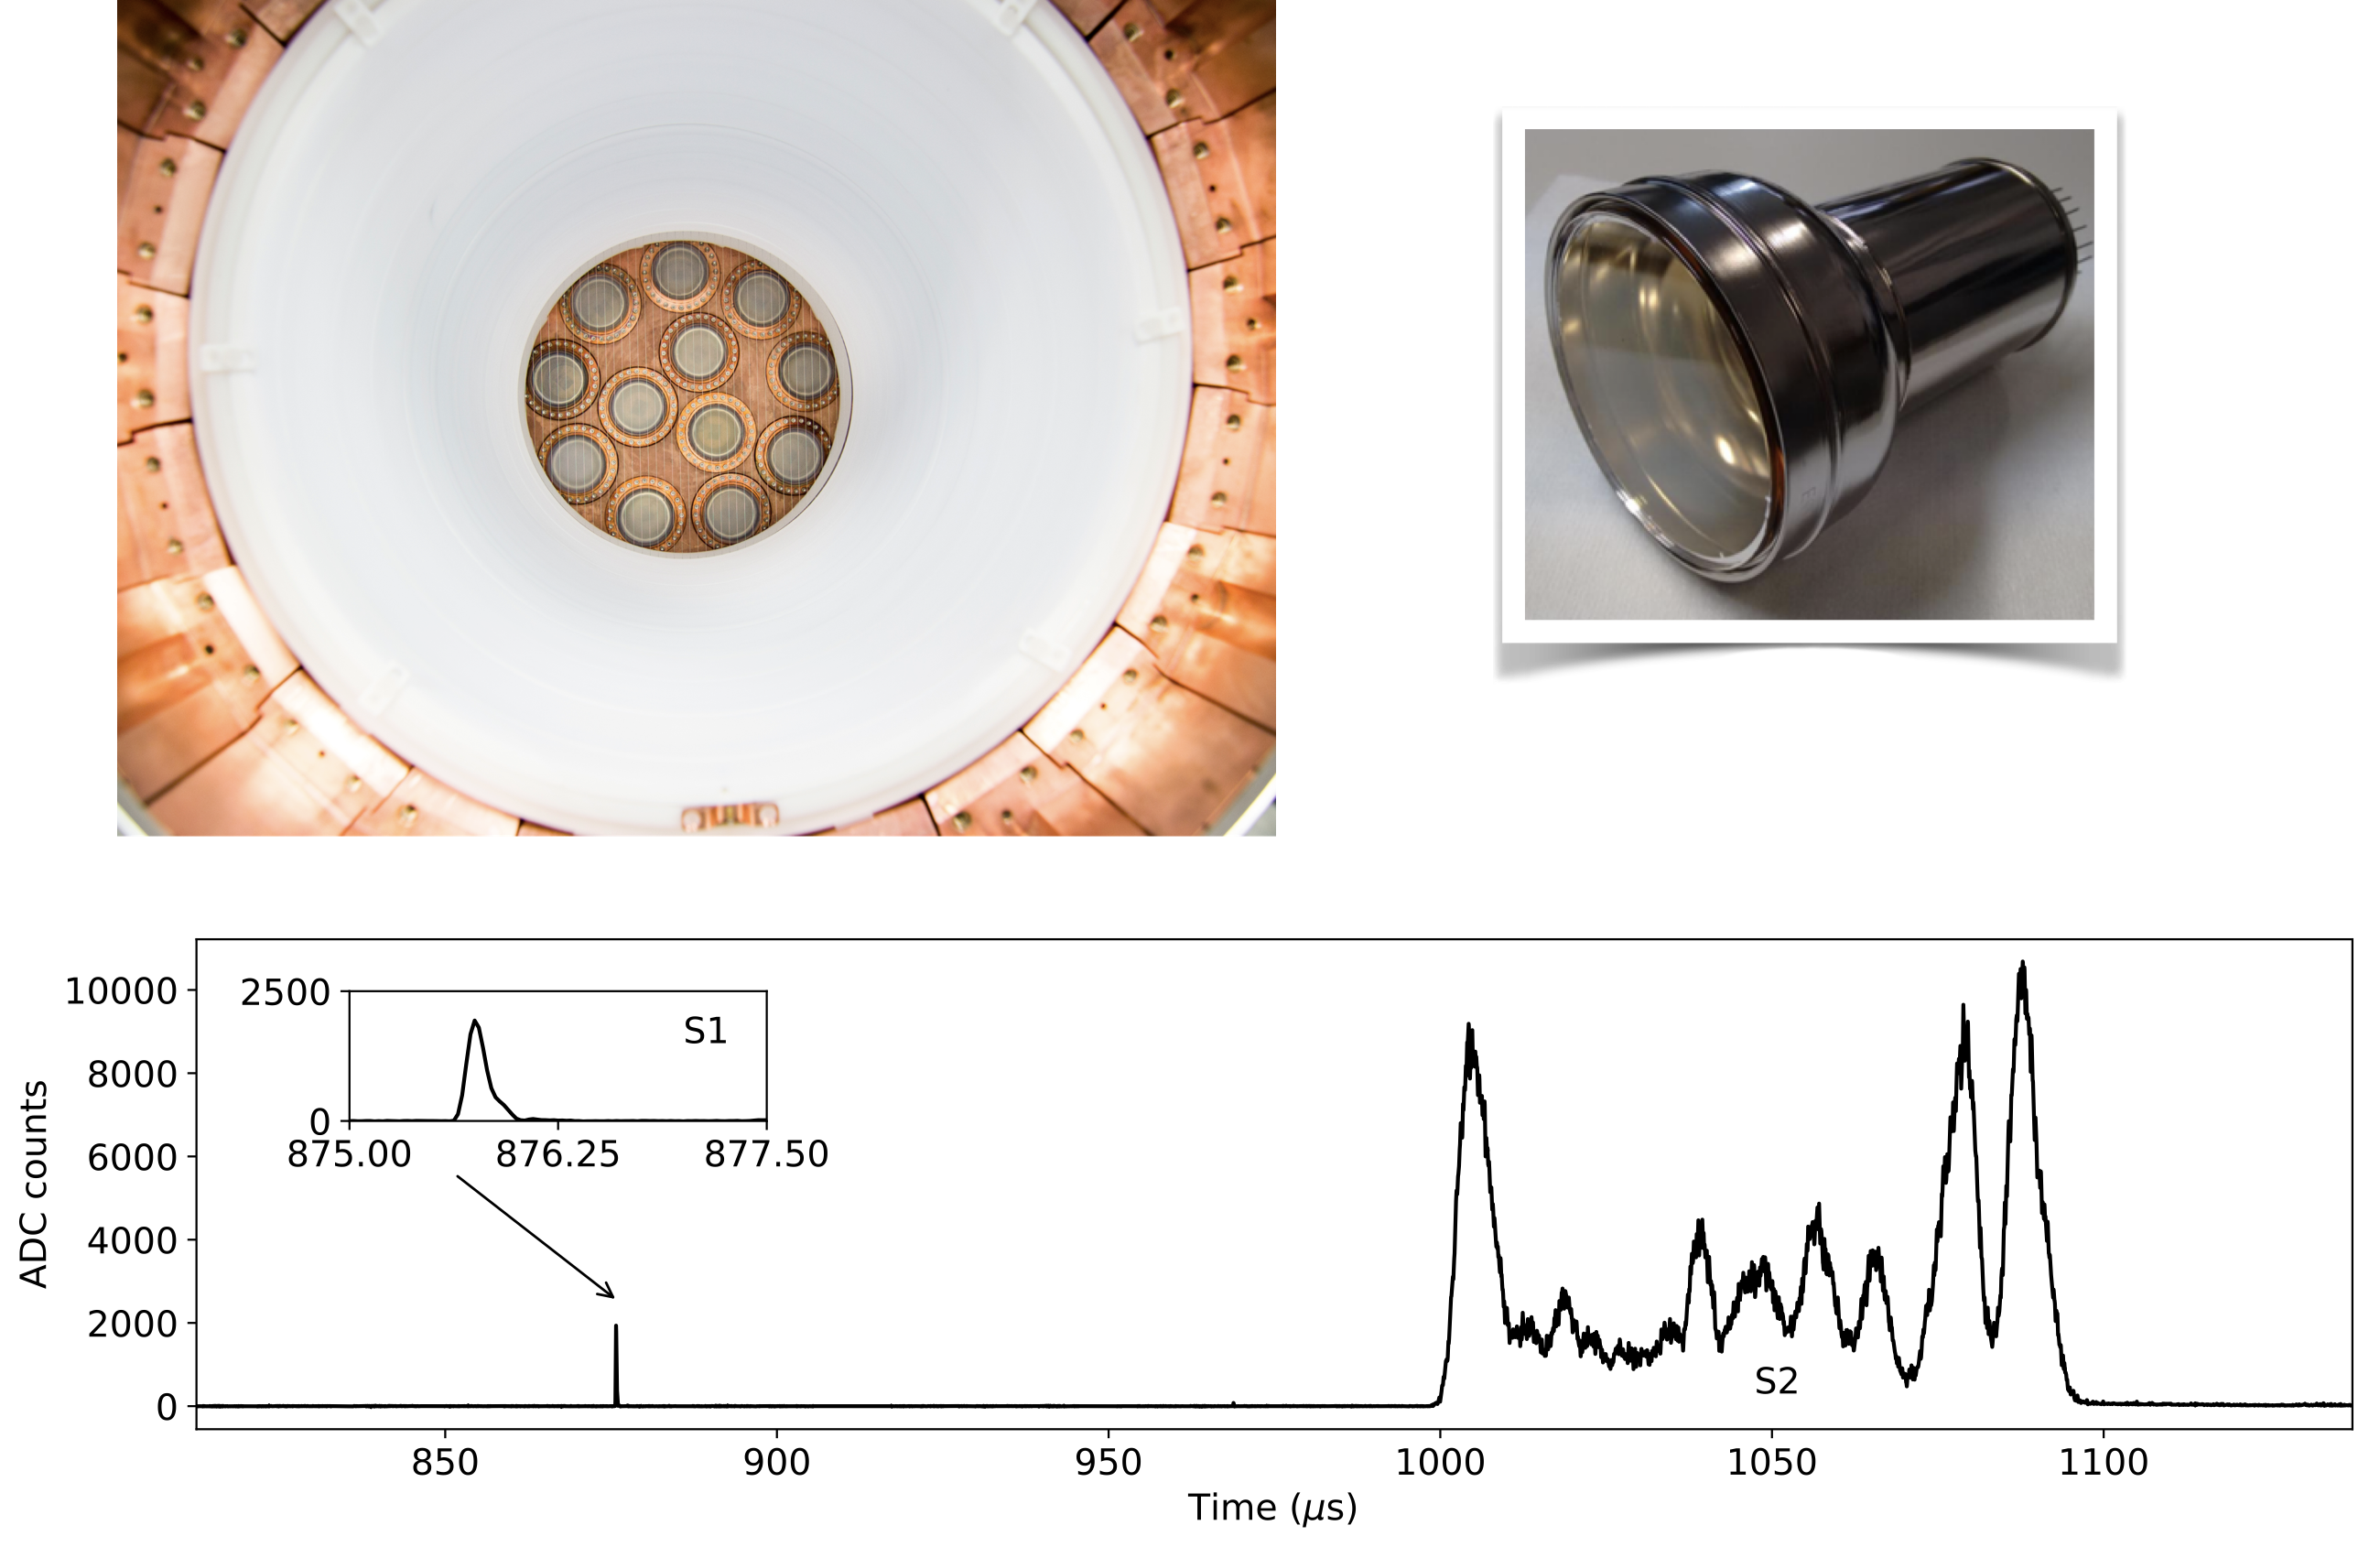
\includegraphics[scale=0.25]{energyPlane.png}

\end{frame}

\begin{frame}{Tracking Plane}

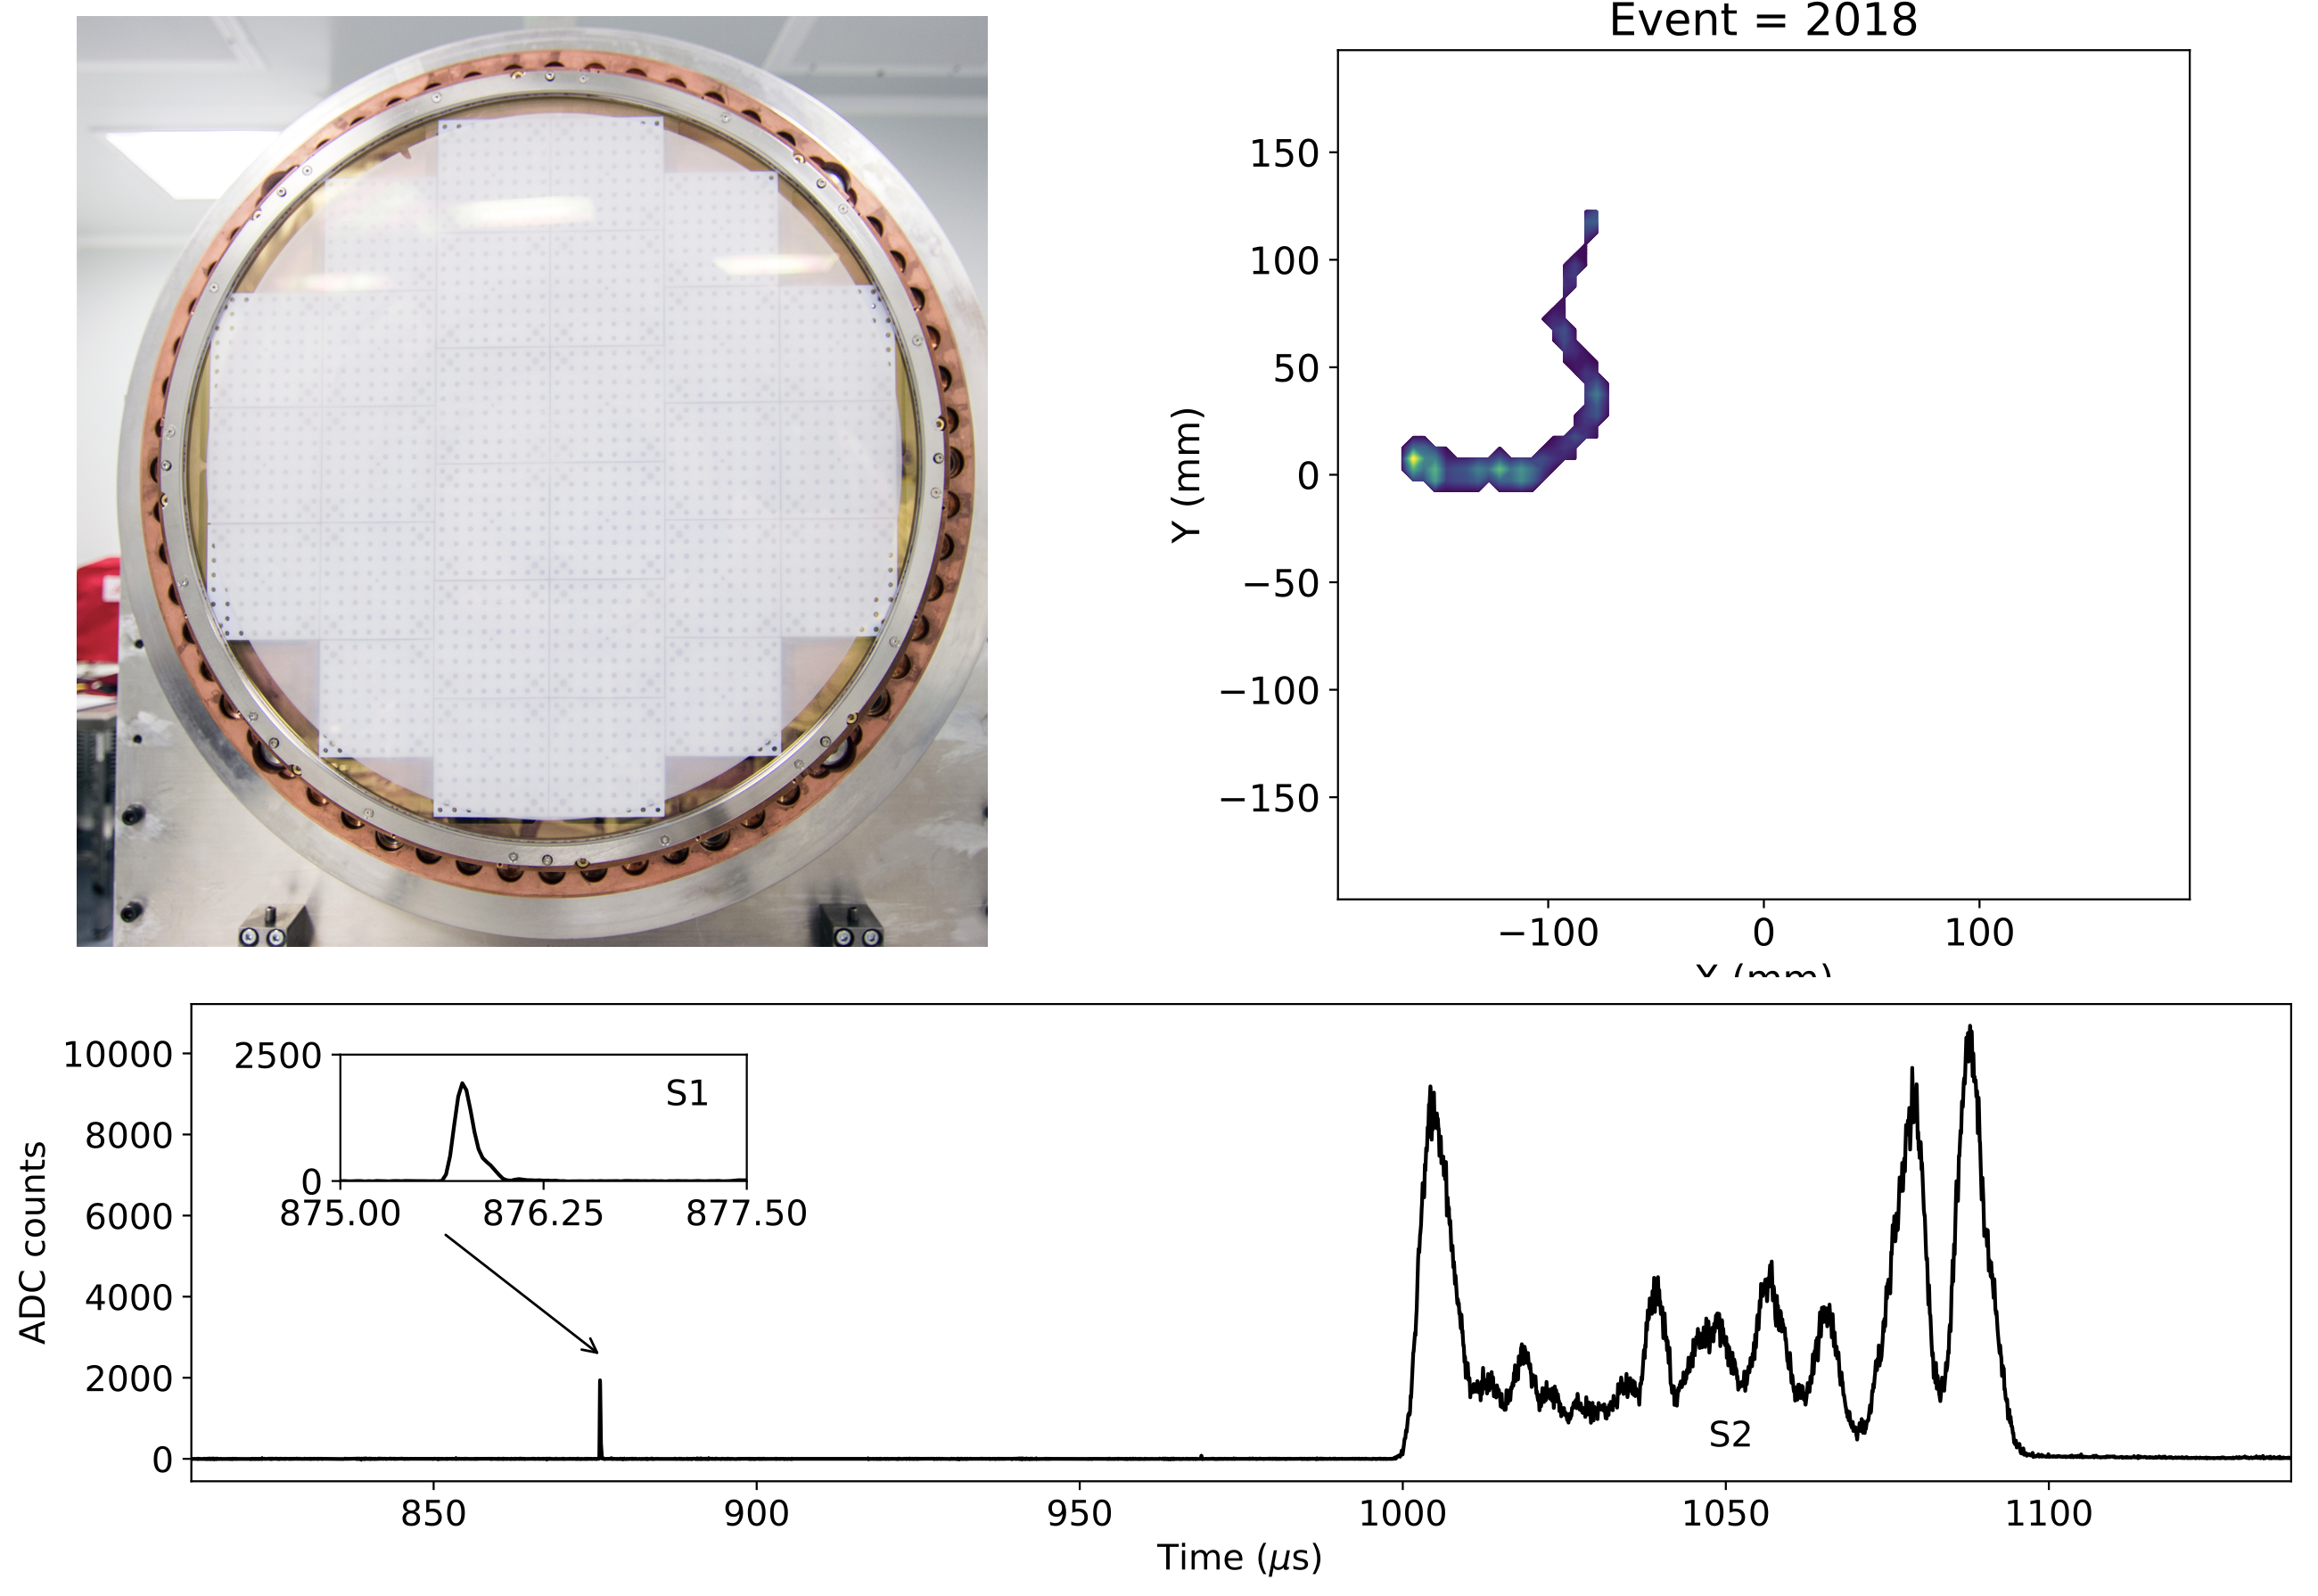
\includegraphics[scale=0.25]{trackinPlane.png}

\end{frame}



\begin{frame}{Detector calibration: Krypton maps}

\begin{columns}
\column{0.50\textwidth}
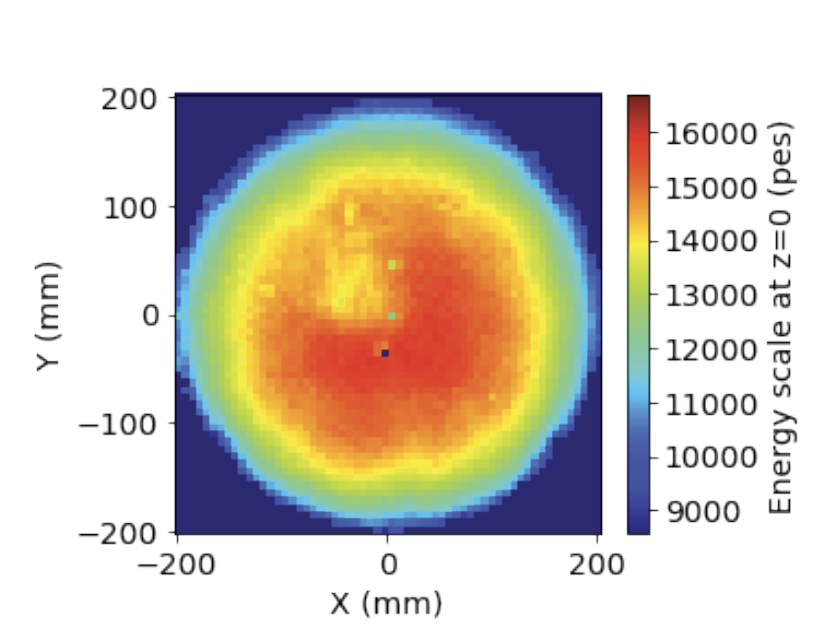
\includegraphics[scale=0.31]{krmaps.png}

 \column{0.50\textwidth}
$\bullet~$ In NEXT, the energy measured by the detector depends on the position (geometrical effect) as well as on the (drifting) electrons lifetime (gas purity). 

$\bullet~$ Both effects can be measured and corrected by flooding the detector with krypton gas (\KR). Each krypton decay leaves a fixed point-like energy deposit ($E_t^{Kr} =43.4$ keV) at a given position $(x,y,z)$ in the detector. A XY map is constructed plotting the ratio $E_o^{Kr}/E_t^{Kr}$ as a function of $(x,y)$. Plotting the same ratio as a function of $z$ gives an exponential that yields the lifetime correction.  
\end{columns}
\end{frame}


%%%
\begin{frame}{Energy resolution in NEXT-White (with Krypton)}

\begin{columns}
\column{0.50\textwidth}
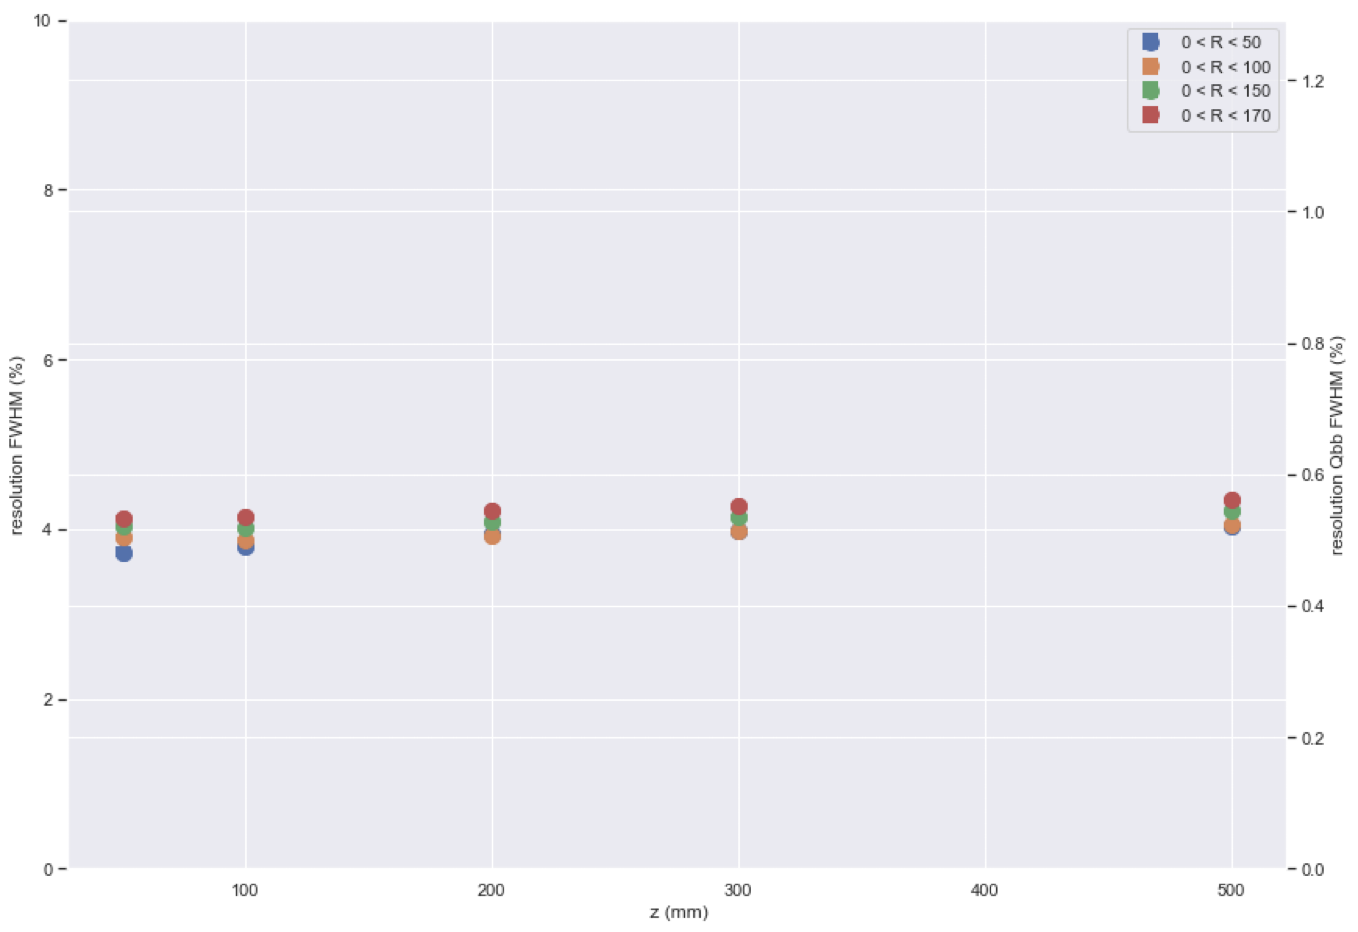
\includegraphics[scale=0.23]{eresKr.png}

 \column{0.50\textwidth}
$\bullet~$ Using \KR, NEXT-White measured an energy resolution of $\sim 4$\% which
extrapolates to $0.5~$\%cat \qbb.

$\bullet~$ This result confirms the early result obtained by DBDM and shows that for point-like
depositions it is possible to reach a value close to intrinsic. 
  
\end{columns}
\end{frame}
%%%
\begin{frame}{Energy resolution in NEXT-White}

\begin{columns}
\column{0.50\textwidth}
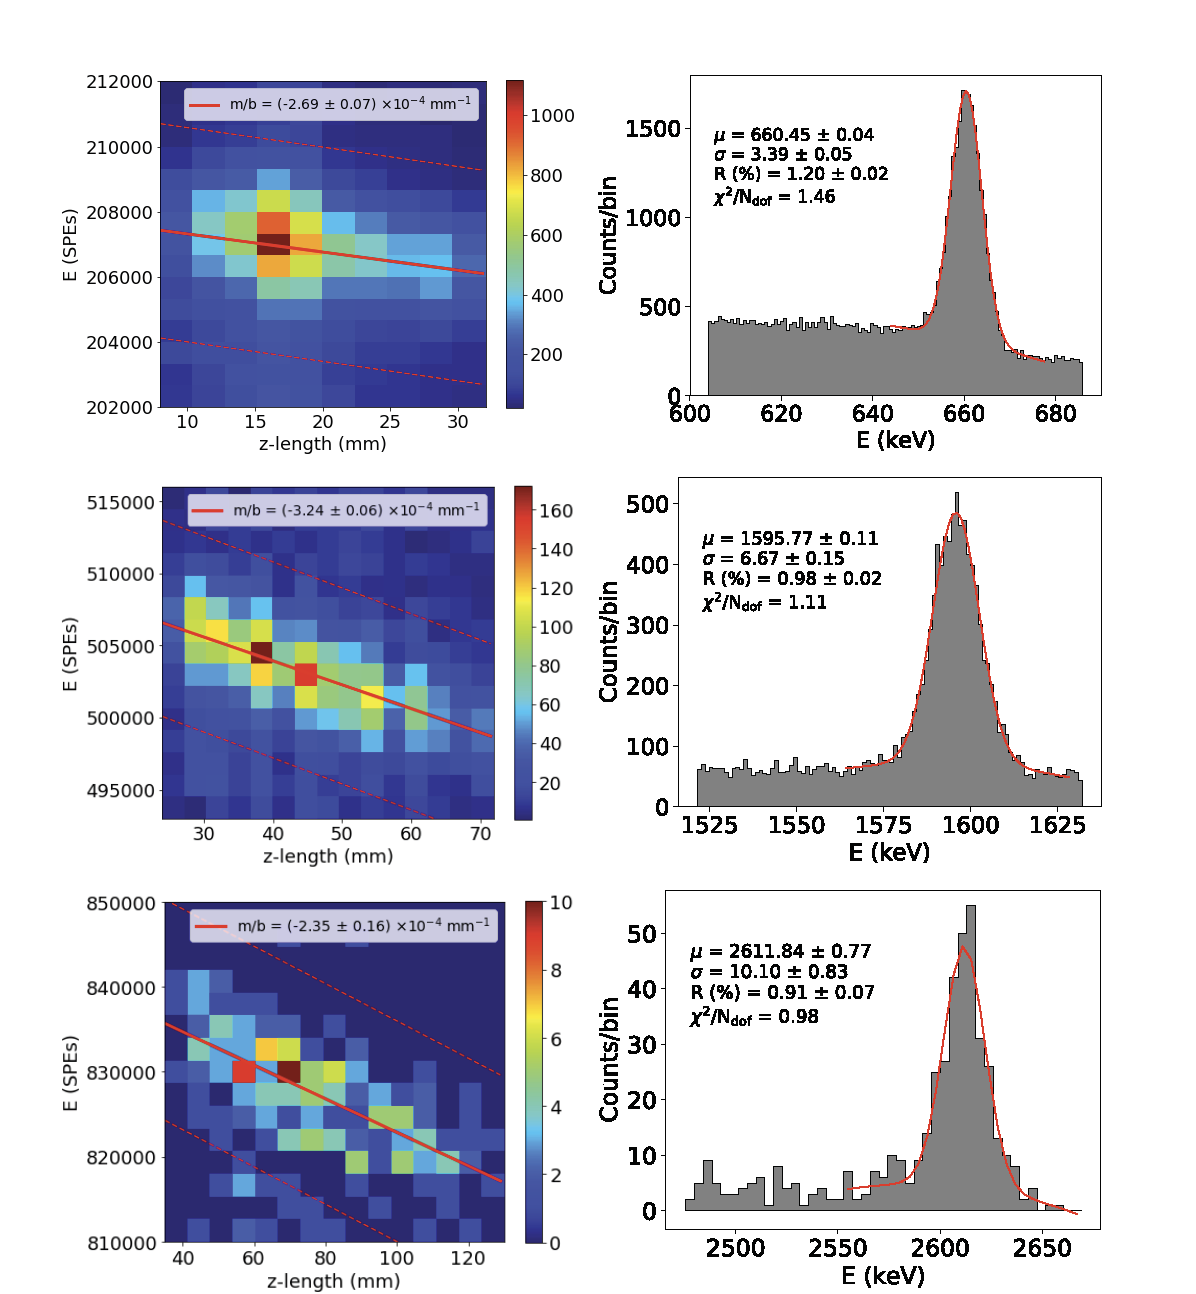
\includegraphics[scale=0.23]{eresWhite.png}

 \column{0.50\textwidth}
$\bullet~$ NEXT-White measured an energy resolution of $\sim 0.9$\% at \qbb.

$\bullet~$ This is a good result, but not as good as the one obtained with DBDM or expected from basic principles. 

$\bullet~$ Possible effects entering the resolution: a) residuals in geometry correction (fix: a more homogenous ``energy plane''); b) residual associated to the lifetime, which in NEXT-White was of the order of several ms (fix: longer lifetime); c) residual associated to track length (fix: shorter tracks?) 
  
\end{columns}
\end{frame}


\begin{frame}{Topological signature: Unblurring}

$\bullet~$ The two blurring effects in the topological signature (diffusion and EL spread) can be characterised using $^{83m}$Kr data in NEXT-White. 

$\bullet~$ Both electron diffusion and the EL light spread can be quantified in terms of point spread functions. The full diffusion PSF is three dimensional: a point-like initial electron cloud transforms after diffusion to an oblate 3D Gaussian (wider in the transverse plane than along the drift direction), where both the transverse and longitudinal widths are proportional to $\sqrt{z}$. This 3D PSF can be projected on the $xy$ plane to yield an effective 2D transverse diffusion PSF. 

$\bullet~$ Similarly, integrating the total light hitting the tracking plane for a point-like charge crossing the EL gap produces a 2D EL PSF. Unlike the diffusion PSF, the EL PSF does not depend on the drift distance $z$.

\end{frame}

\begin{frame}{EL-PSF}

\begin{columns}
\column{0.50\textwidth}
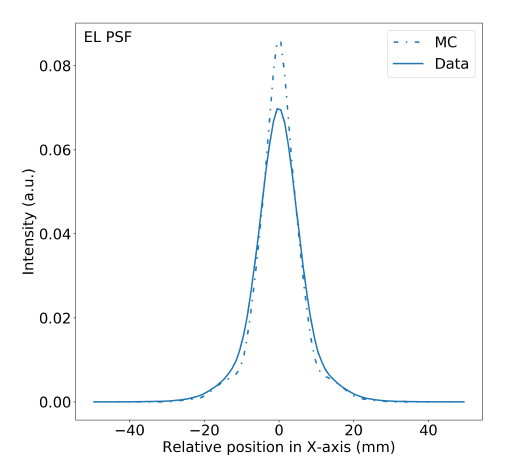
\includegraphics[scale=0.40]{ELPSF.png}
 \column{0.50\textwidth}

$\bullet~$EL PSF can be determined from $^{83m}$Kr events occurring immediately in front of the gate, such that they do not suffer a diffusive spread and can be considered point-like. The procedure involves recording a large number of $^{83m}$Kr events over a small drift region (drift time $<25\;\mu$s). For each event, the SiPM response is integrated over several $\mu$s, to include the full S2 signal. The $xy$ location of the event is determined by calculating the center of gravity (COG) of the SiPM hit map. 

$\bullet~$ In NEXT-White, the MC does not fully reproduce the data (no surprise: modelling the optical behaviour of the TPC is difficult), but the PSF can be extracted from the data themselves. 
\end{columns}
\end{frame}

\begin{frame}{ Diffusion PSF and combination}

\begin{columns}
\column{0.50\textwidth}
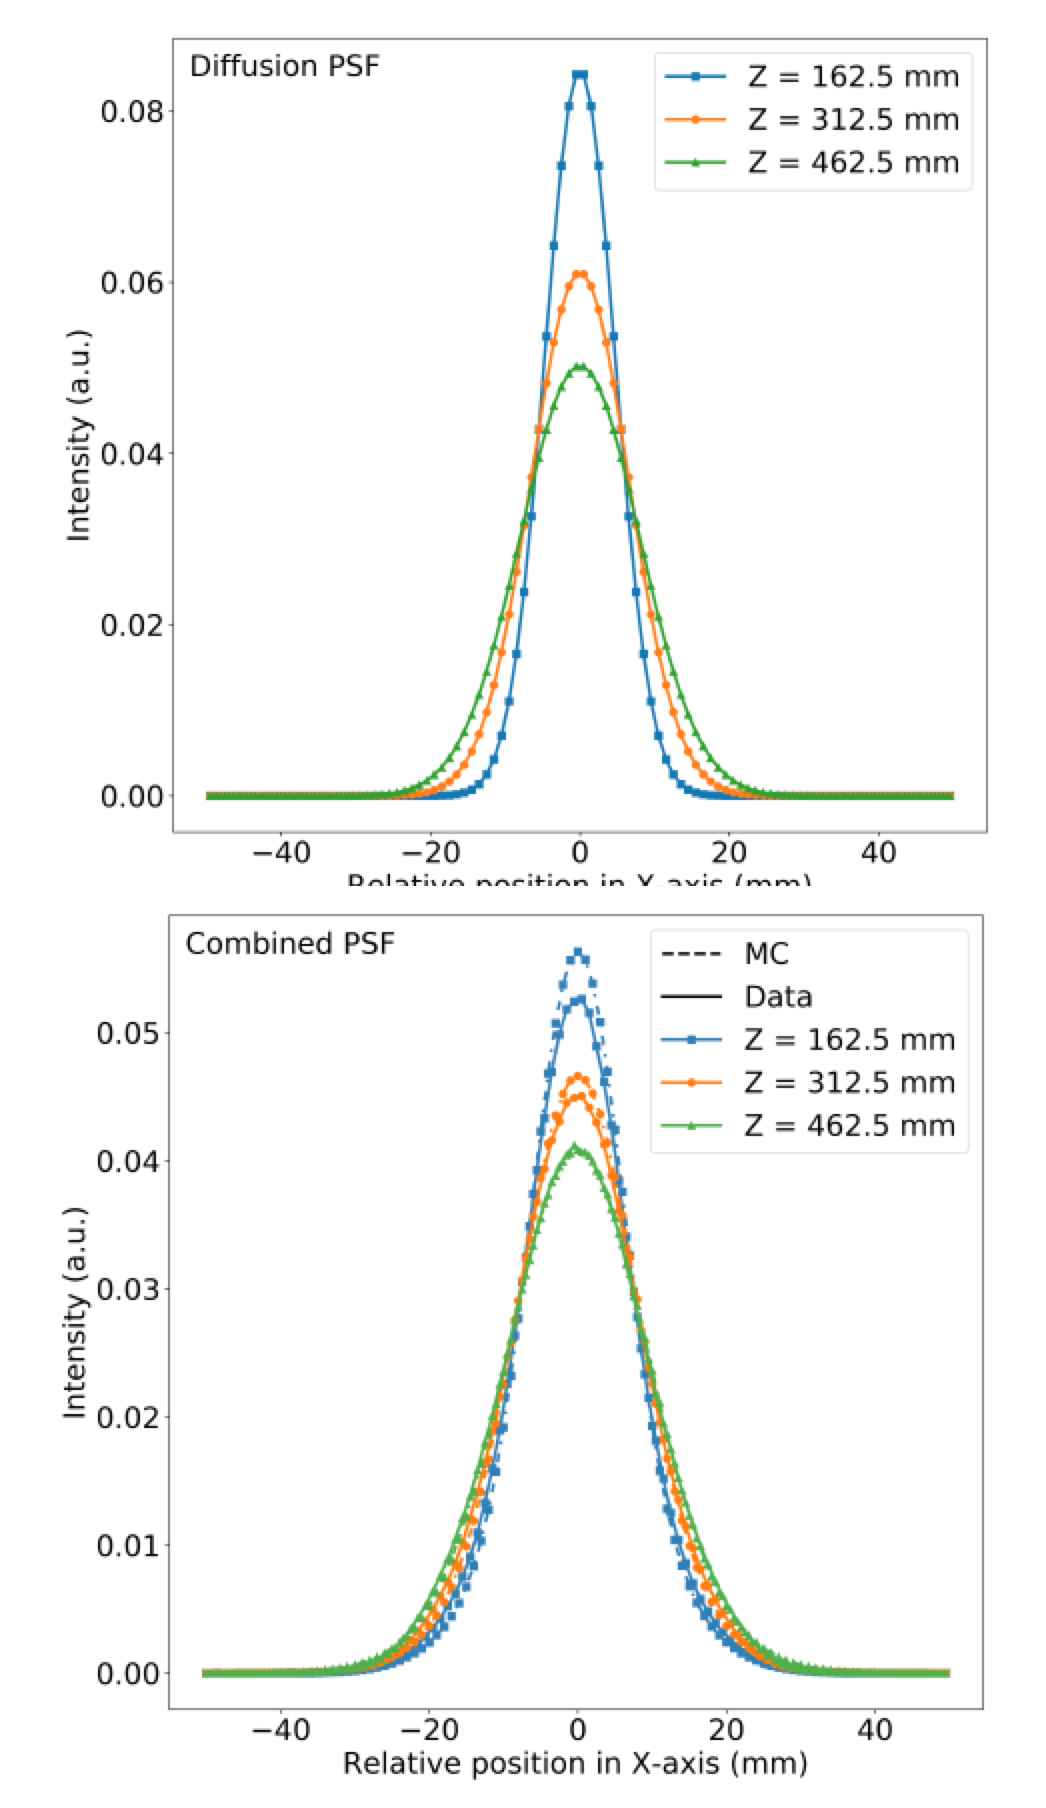
\includegraphics[scale=0.25]{combinedPSF.png}
 \column{0.50\textwidth}

$\bullet~$The effective 2D transverse diffusion PSF is given approximately by a Gaussian whose standard deviation is: $\sigma_t=1.07\sqrt{z}$, where $z$ is in cm and $\sigma_t$ in mm. 

$\bullet~$ The two blurring effects of diffusion and EL light production can be combined in a single z-dependent PSF, which, to a good approximation, is given by their convolution: $F_{dif+EL}(z)=F_{dif}^{2D}(z) * F_{EL}$.  The combined PSF can be determined experimentally similarly to the EL PSF, by selecting $^{83m}$Kr events over a range $[z,z+\Delta z]$
\end{columns}
\end{frame}

 \begin{frame}{Richardson-Lucy (RL) deconvolution algorithm }

$\bullet~$ The Richardson-Lucy (RL) algorithm aims to recover, by deconvolution, an underlying sharp image from an observed blurred and noisy one. The algorithm is iterative, generating a sequence of improved approximations for the underlying image using the (presumably known) point spread function (PSF) of the imaging process.

$\bullet~$ We denote by $W(x,y)$ the underlying sharp image and by $F(x,y)$ the PSF. In the absence of noise, the blurred image $H(x,y)$ is obtained as a convolution of $W$ and $F$:

\begin{equation}
H(x,y)=\iint W(x',y') F(x-x',y-y') dx' dy' \label{eq: H ideal}
\end{equation}

$\bullet~$ In principle, $W(x,y)$ can be recovered from $H(x,y)$ by solving this integral equation. This could be done by discretisation, converting $H$, $W$ and $F$ into matrices and the integral to a double summation. This generates a system of linear equations with the elements of $W$ as the unknowns:

\begin{equation}
\sum_{j}^{} F_{i,j}W_j = H_i \label{eq: linear equation system with H} 
\end{equation} 

 \end{frame}
 
 \begin{frame}{Deconvolution: the problem of noise}
$\bullet~$  In reality, because of the presence of noise, the actual observed image $\tilde{H}(x,y)$ is different from the ideal one $H(x,y)$. The system of linear equations then becomes:

\begin{equation}
\sum_{j}^{} F_{i,j}W_j = \tilde{H}_i \label{eq: linear equation system with H tilde} 
\end{equation} 

$\bullet~$  Attempting to solve equations (\ref{eq: linear equation system with H tilde}) generally yields poor results, with large discontinuities in $\{W_j\}$, as well as non-physical negative values. This occurs because the process tends to amplify short-wavelength errors in $\tilde{H}$, which are characteristic of noisy images. 

 \end{frame}

\begin{frame}{RL: The iterative approach}
$\bullet~$  The approach RL algorithm begins by noting that one could formally write:  

\begin{equation}
W(x,y)=\iint H(x',y') G(x-x',y-y') dx' dy' \label{eq: direct inversion}
\end{equation}
provided that we define the inverse kernel $G$ as:

\begin{equation}
G(x-x',y-y')=\frac{W(x,y) F(x-x',y-y')}{H(x',y')} \label{eq: G ideal}  
\end{equation}
where $\iint F(x-x',y-y') dx' dy' = 1$. Since $G$ depends on $W$, the direct calculation of $W$ from equation (\ref{eq: direct inversion}) is impossible. However, the process may work iteratively, if one could provide successively improved approximations for $G$, which, in turn, would rely on successive estimates of $W$. 

 \end{frame}
 
\begin{frame}
We begin with an initial estimate $W^{(0)}$ for $W$, where $W^{(0)}(x,y)$ is generally taken to be a flat image. In the $r$-th iteration we calculate an intermediate blurred image $H^{(r)}$ by:

\begin{equation}
H^{(r)}(x,y)=\iint W^{(r)}(x',y') F(x-x',y-y') dx' dy' \label{eq: H(r)}
\end{equation}   
This allows finding an estimate for $G$:

\begin{equation}
G^{(r)}(x-x',y-y')=\frac{W^{(r)}(x,y) F(x-x',y-y')}{H^{(r)}(x',y')} \label{eq: G(r)}  
\end{equation}

The new estimate for $W$, $W^{(r+1)}$, is then calculated following equation (\ref{eq: direct inversion}), with $\tilde{H}$ replacing $H$ and $G^{(r)}$ replacing $G$:

\begin{equation}
\begin{split}
W^{(r+1)}(x,y) &= \iint \tilde{H}(x',y') G^{(r)}(x-x',y-y') dx' dy' \\
&= W^{(r)}(x,y) \iint \frac{\tilde{H}(x',y')}{H^{(r)}(x',y')} F(x-x',y-y') dx' dy' \label{eq: W(r)}
\end{split}
\end{equation}

If successive changes in $W^{(r)}$ are sufficiently small, in the limit $r \rightarrow \infty$ the scheme converges to the solution of the corresponding maximum likelihood problem.

\end{frame}
\begin{frame}{RL implementation in NEXT-White: Conceptual}

$\bullet~$ In NEXT-White, RL deconvolution is applied on individual SiPM time-sliced hit maps (each integrated over a time interval $\delta t=2$\;$\mu$s). The recipe is as follows:
\begin{enumerate}
\item {\color{uwopurple} For a slice recorded at time $t$, associate a physical slice of width $\delta z=v_d\delta t$ of the original 3D track to the corresponding drift distance $z=v_d\cdot(t-t_0)$ (for $v_d=0.9$\;mm/s, $\delta z=1.8$\;mm). }
\item  {\color{uwopurple}  Identify the physical slice with the underlying sharp 2D image $W(x,y)$, and the corresponding SiPM hit map as a sampled representation of the blurred image $\tilde{H}(x,y)$.}
\item  {\color{uwopurple} The two images are assumed to be related through the combined diffusion+EL PSF $F(x,y;z)$ corresponding to a drift distance $z$. }
\end{enumerate}

\end{frame}

\begin{frame}{Deconvolution of \KR\ events}

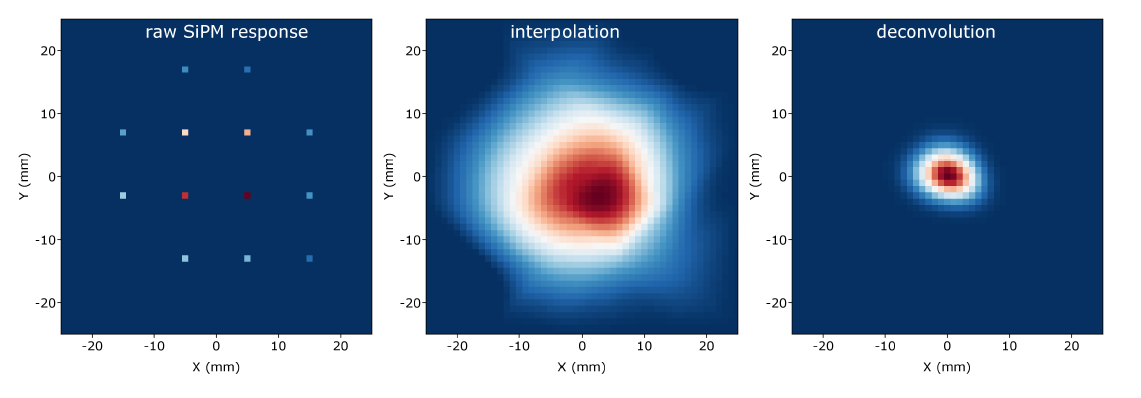
\includegraphics[scale=0.27]{psfint.png}

\begin{enumerate}
	
	{\color{uwopurple} \item Charge cut: SiPMs with $q < 10$~PE  are removed from the slice.} 
	{\color{uwopurple} \item 2D interpolation: Define a rectangular region surrounding the SiPMs which have survived charge cut. Apply bicubic 2D interpolation on the  SiPM hit map.}
	{\color{uwopurple} \item RL deconvolution: For each slice, we use the corresponding z-dependent combined EL+diffusion PSF for the deconvolution process. }
\end{enumerate}
\end{frame}

\begin{frame}{Deconvolution of tracks}

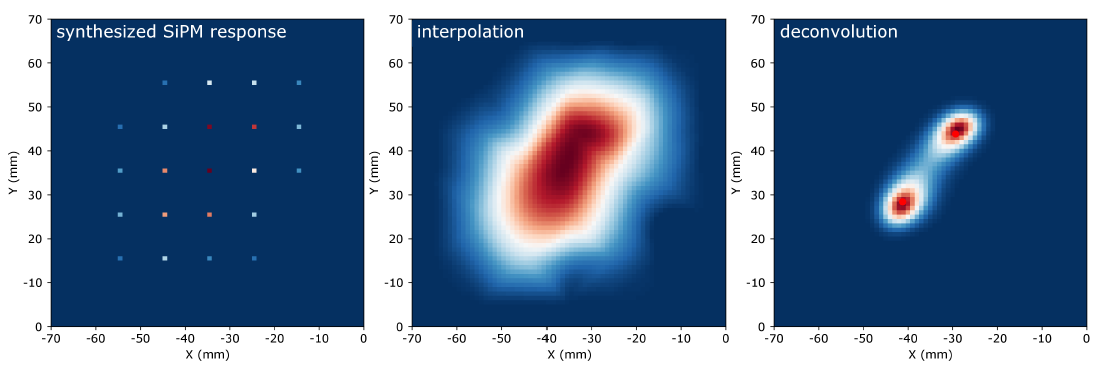
\includegraphics[scale=0.27]{decon2kr.png}

$\bullet~$ A track can be viewed as a set of point-like Kr-events. Thus applying the procedure on a slice-by-slice basis, yields the track deconvolution. In this example, we deconvolve two Kr depositions. 
\end{frame}

\begin{frame}{Recovering the topological signature}
\begin{columns}
\column{0.60\textwidth}
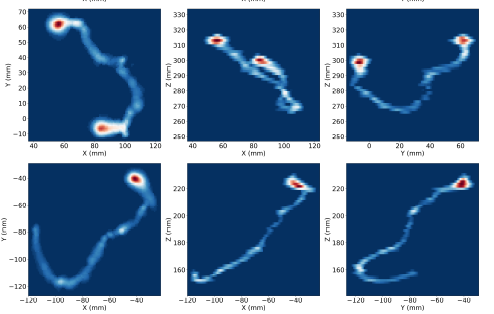
\includegraphics[scale=0.50]{deconv1e2e.png}
 \column{0.40\textwidth}

$\bullet~$ After deconvolution, we can recover a clean topological signature (1e vs 2e), in spite of diffusion (these are real data electrons and double electrons from the 1.6 MeV double escape peak of \TL) 
 \end{columns}
\end{frame}

\begin{frame}{Applying the topological signature}
%\begin{columns}
%\column{0.60\textwidth}
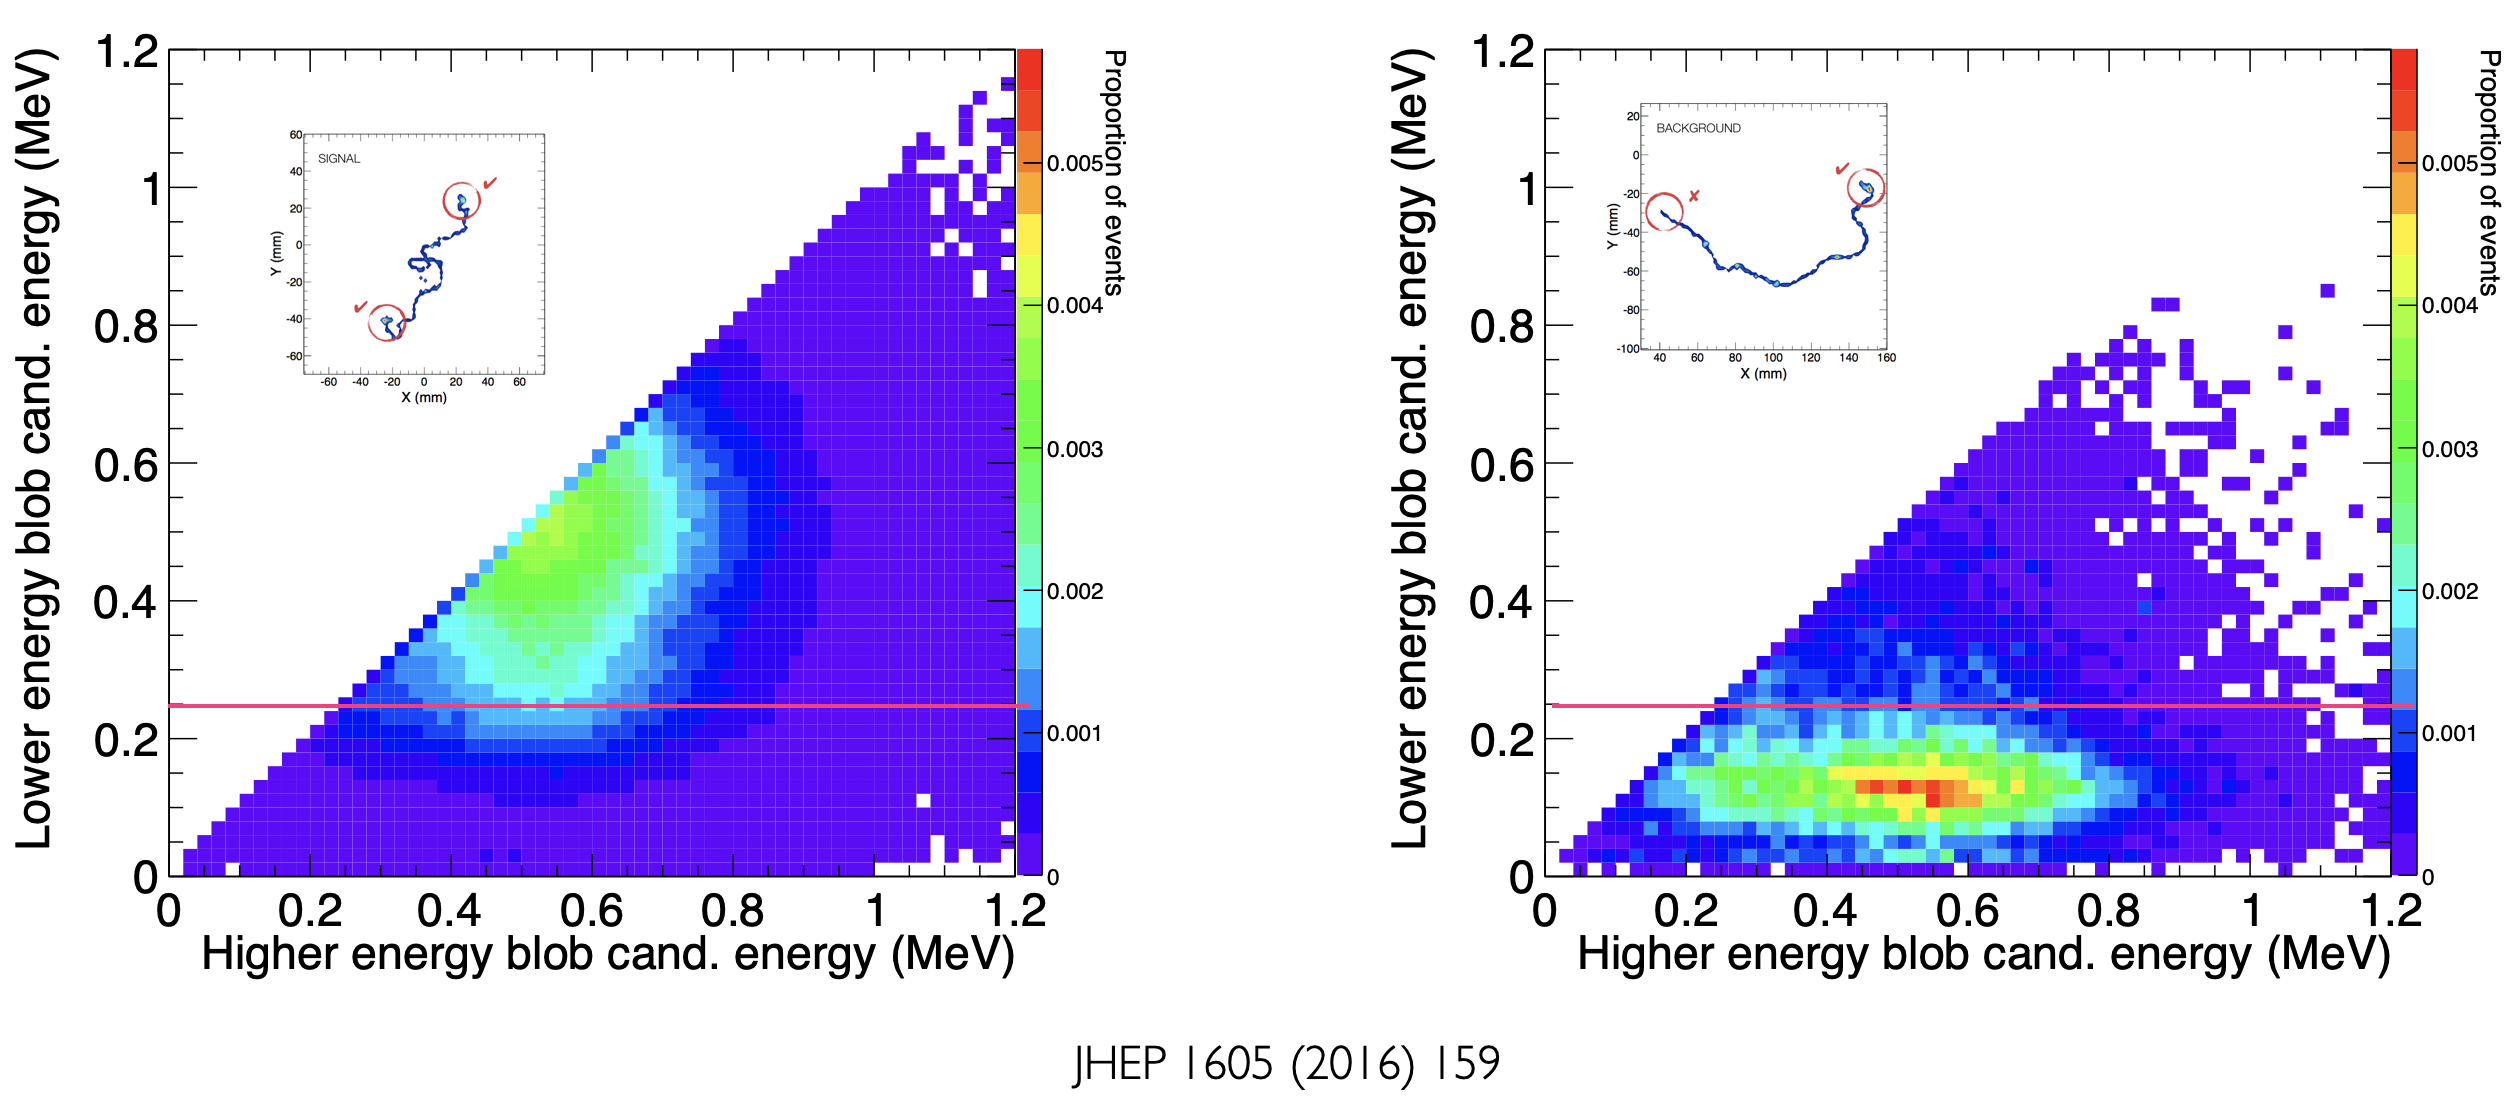
\includegraphics[scale=0.30]{topoNew.png}
 %\column{0.40\textwidth}

%$\bullet~$ After deconvolution, we can recover a clean topological signature (1e vs 2e), in spite of diffusion (these are real data electrons and double electrons from the 1.6 MeV double escape peak of \TL) 
 %\end{columns}
\end{frame}

\begin{frame}{Energy Spectrum}
\begin{columns}
\column{0.60\textwidth}
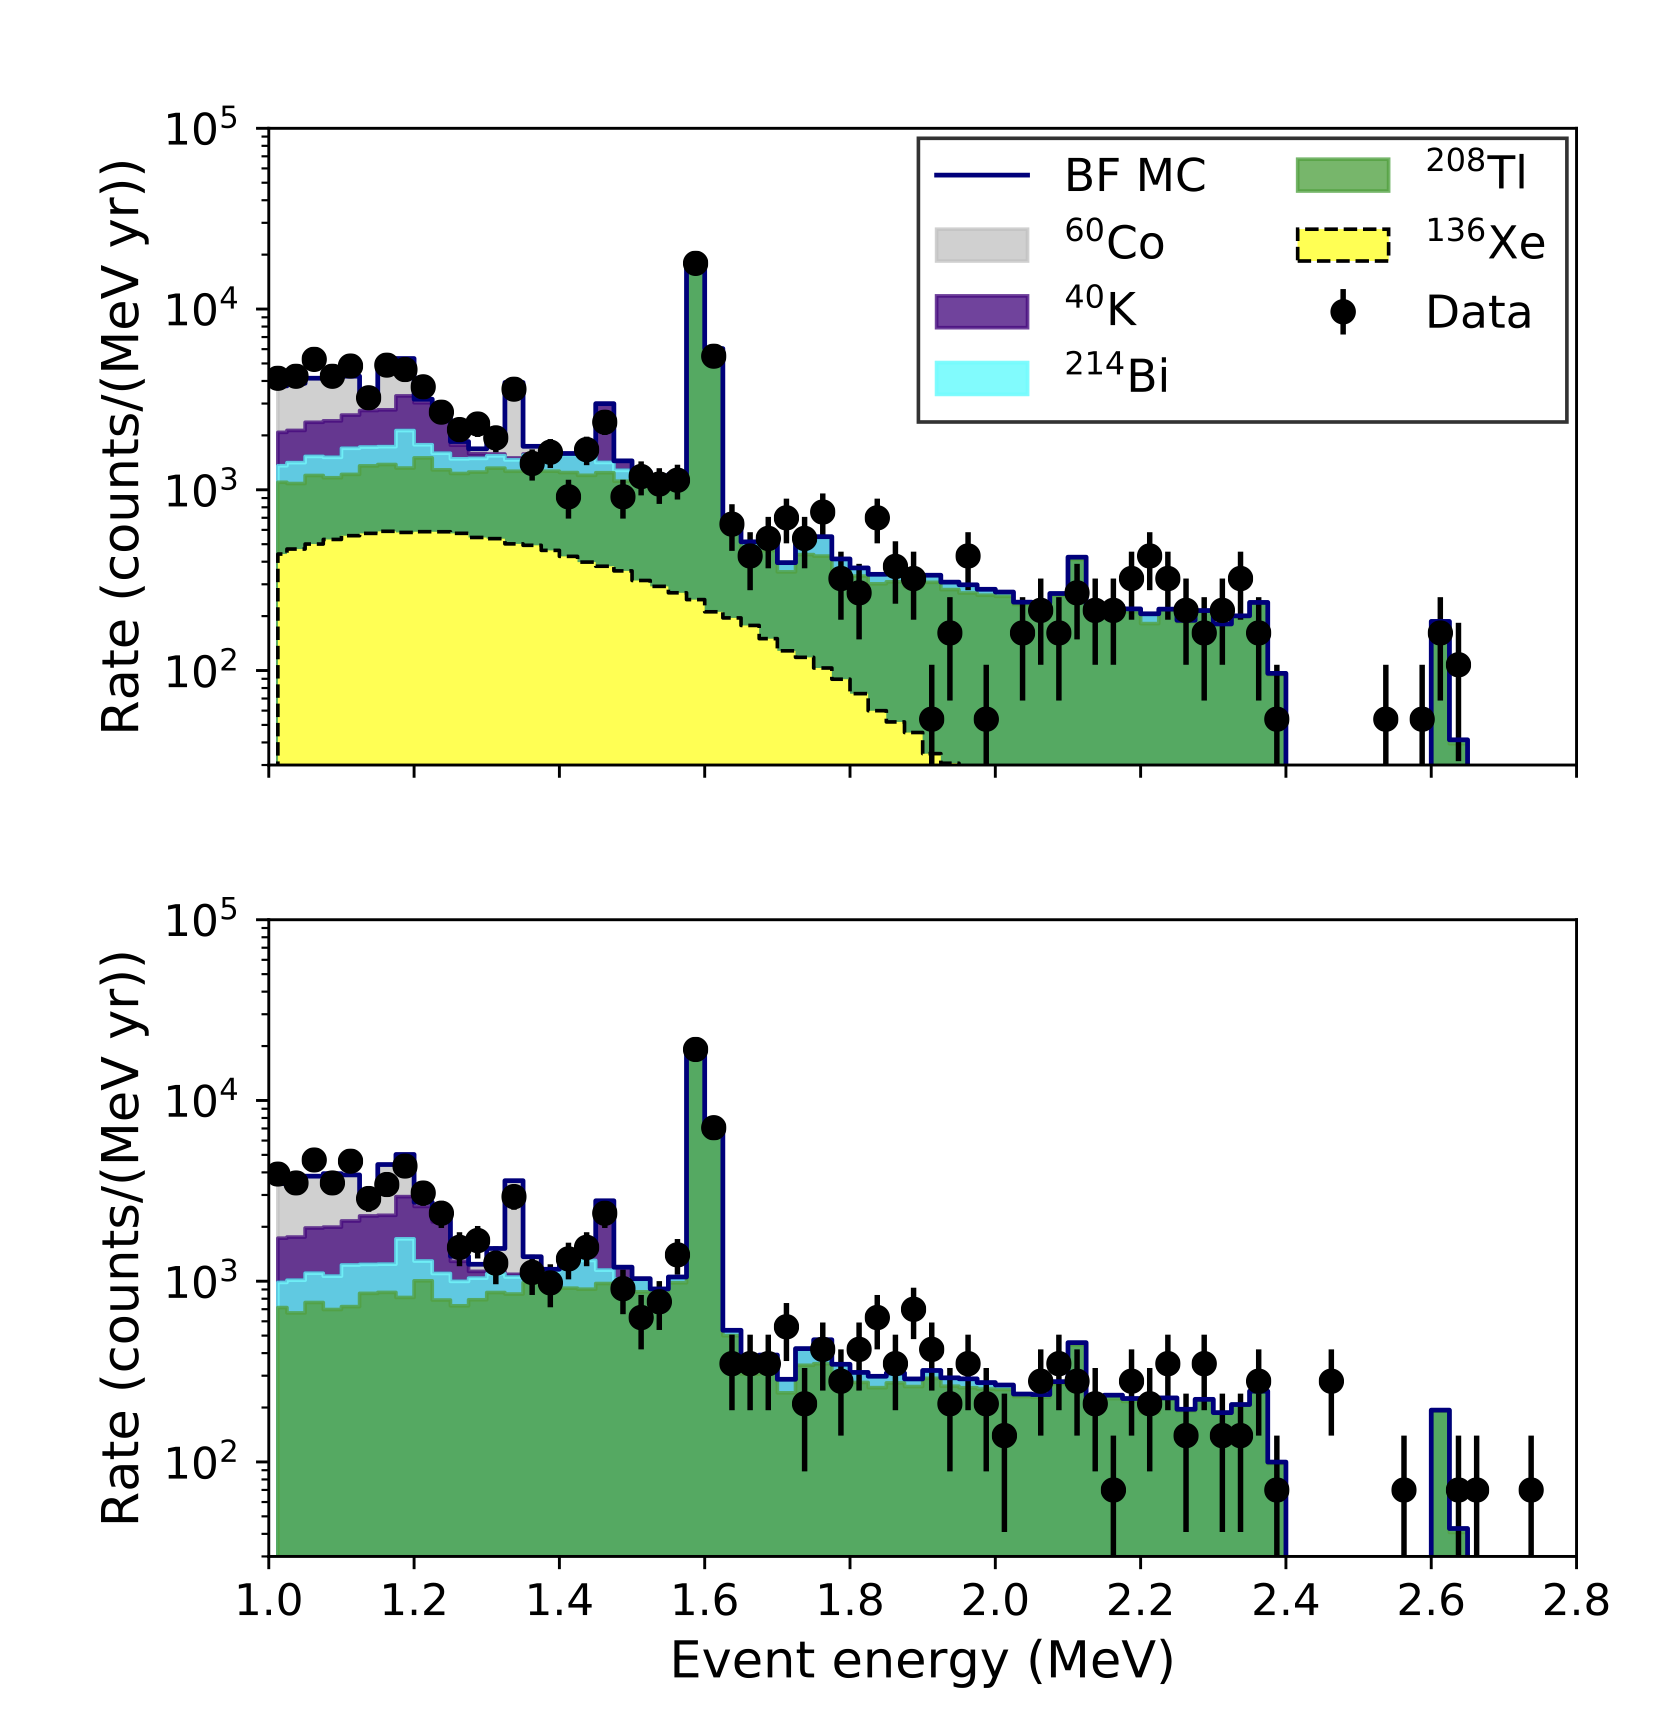
\includegraphics[scale=0.26]{newSpectrum.png}
\column{0.40\textwidth}

$\bullet~$ Energy spectrum measured by NEXT-White. A Xenon TPC like NEXT can run with depleted xenon (no \XE) and with enriched xenon (90\% of \XE) and compared results, thus reducing very much the dependence with the Monte Carlo. 

$\bullet~$ Notice the hole around \qbb, where a putative signal may show up. 
 \end{columns}
\end{frame}

\begin{frame}{\bbtnu\ mode}
\begin{columns}
\column{0.60\textwidth}
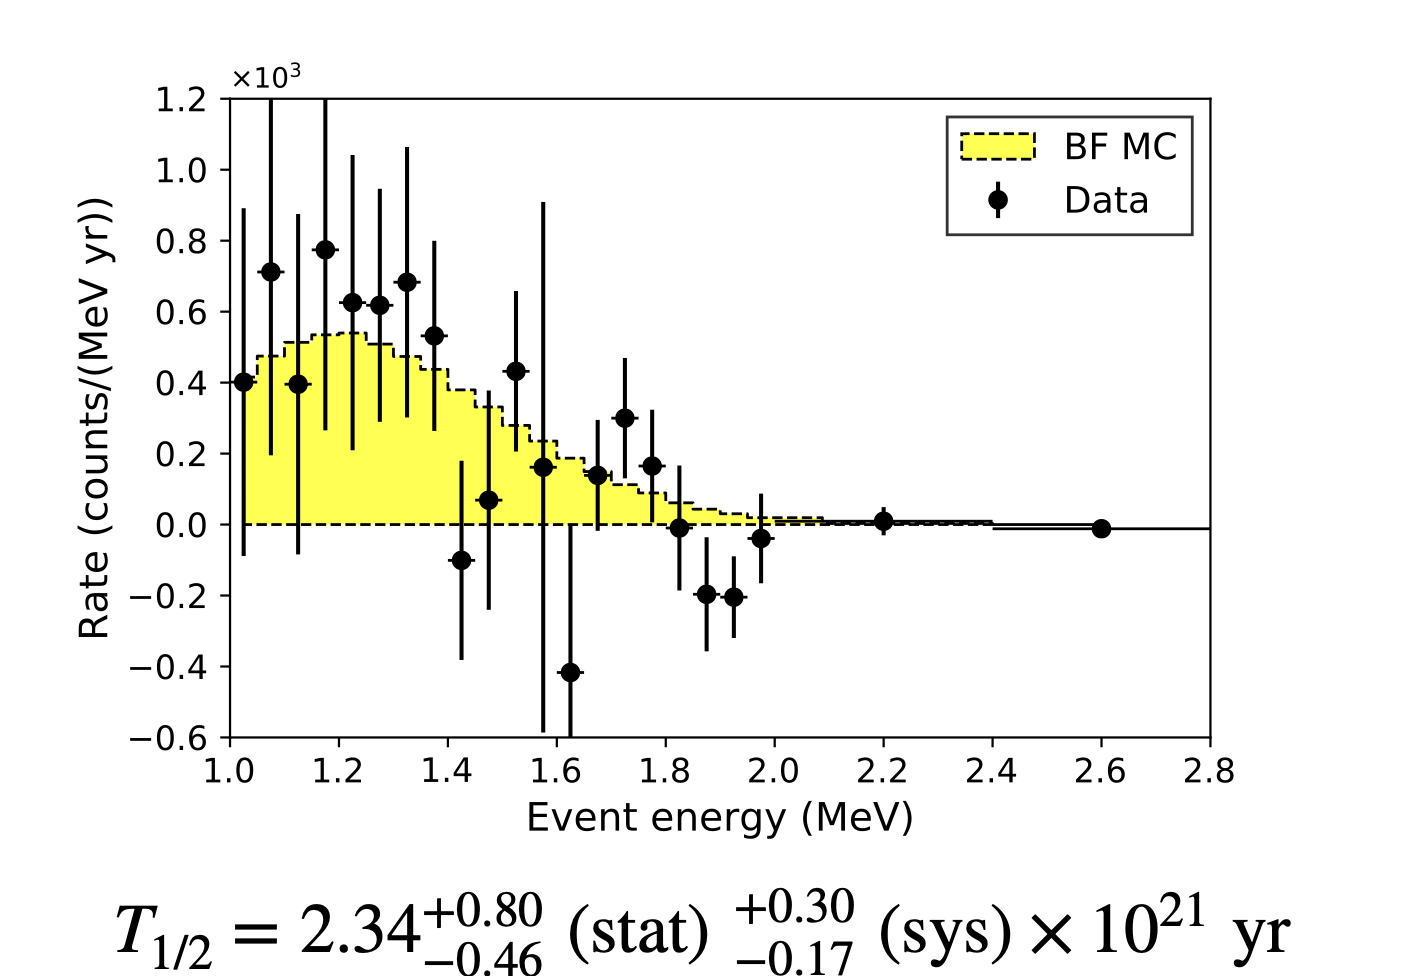
\includegraphics[scale=0.36]{bb2nu.png}
\column{0.40\textwidth}

$\bullet~$ Although NEXT-White is a relatively small detector (5 kg of active volume), it has been able to measure the \bbtnu\ mode (St. Gotthard TPC, with a similar mass couldn't do it, due to backgrounds). 

$\bullet~$ In particular, in NEXT-White has been possible to measure the \bbtnu\ mode using direct subtraction between the data with enriched and depleted xenon. 
 \end{columns}
\end{frame}

%\begin{frame}{Sailing to Ithaca}
%\begin{columns}
%\column{0.50\textwidth}
%\includegraphics[scale=0.18]{francesDemo.png}
%
%Francesc (then grad student) working in NEXT-DEMO, circa 2012
%
%\column{0.50\textwidth}
%\includegraphics[scale=0.17]{FrancescNew.png}
%
%Francesc (now NEXT TC) in NEXT-White, circa 2022
% 
% \end{columns}
%\end{frame}









%%%
\end{document}